\documentclass[11pt]{article}



\usepackage[utf8]{inputenc} % Required for inputting international characters
\usepackage[T1]{fontenc} % Output font encoding for international characters
\usepackage{graphicx}
\usepackage{float}
\usepackage{geometry}
\usepackage{hyperref}
\usepackage{amsmath}
\usepackage{cite}
\usepackage{pdfpages}
\usepackage{caption} 
\usepackage{subcaption}
\captionsetup[table]{position=above,skip=0.7cm} 
\newcommand{\RM}[1]{\MakeUppercase{\romannumeral #1{}}}
\makeatletter
\newcommand*{\rom}[1]{\expandafter\@slowromancap\romannumeral #1@}
\makeatother

\usepackage{adjustbox}
\usepackage[german]{varioref}
\usepackage{mathpazo} % Palatino font
\usepackage[german]{babel}
\parindent0pt
\pdfinclusioncopyfonts=1

\begin{document}

\begin{titlepage} % Suppresses displaying the page number on the title page and the subsequent page counts as page 1
	\newcommand{\HRule}{\rule{\linewidth}{0.5mm}} % Defines a new command for horizontal lines, change thickness here
	
	\center % Centre everything on the page
	\vspace*{0.75cm}
%
\includegraphics[width=0.8\textwidth]{../tex/fu_logo}\\[1cm] 

%\textsc{\LARGE  Freie Universität Berlin}\\[1.5cm] % Main heading such as the name of your university/college
	
	\textsc{\Large Neurobiologie für BioinformatikerInnen: Praktikum B}\\[0.65cm] % Major heading such as course name
	
	\textsc{\large Protokoll zum 5. Praktikumstag am 04.02.2019}\\[0.65cm] % Minor heading such as course title

	\HRule\\[0.5cm]
	
	{\huge Psychophysische Experimente zum \\[0.2cm]Farbensehen}\\[0.3cm] % Title of your document
	
	\HRule\\[0.75cm]
	\textsc{\Large\bfseries Gruppe \RM{4}}
	\\[0.8cm]
	
\vfill

	\begin{minipage}{0.45\textwidth}
		\begin{flushleft}
			\large
			\textit{Gruppenmitglieder}\\
			\textsc{Alia Rothkegel}\\
			\textsc{Mara Steiger}
			 % Your name
		\end{flushleft}
	\end{minipage}
	~
	\begin{minipage}{0.45\textwidth}
		\begin{flushright}
			\large \vspace{16pt}
			alia.rothkegel@fu-berlin.de\\
			mara.steiger@fu-berlin.de 
		\end{flushright}
	\end{minipage}
	
\vfill

	\begin{minipage}{0.45\textwidth}
		\begin{flushleft}
			\large
			\textit{Lehrveranstalter}\\
			Prof. Dr. P.R. \textsc{Hiesinger}\\ 
			Dr. D. \textsc{Malun}\\ 
			Prof. Dr. M. \textsc{Wernet}
		\end{flushleft}
	\end{minipage}
	~
		\begin{minipage}{0.45\textwidth}
		\begin{flushright}
			
		\end{flushright}
	\end{minipage}
\vfill
	\begin{minipage}{0.7\textwidth}
		\begin{flushleft}
			\large
			\textit{TutorInnen}\\
			\textsc{Lisa Peters}\\
			\textsc{Johannes Brüner Hammacher}\\
			\textsc{Claudia Haushalter}
		\end{flushleft}
	\end{minipage}
	~
		\begin{minipage}{0.2\textwidth}
		\begin{flushright}
			
		\end{flushright}
	\end{minipage}

	% If you don't want a supervisor, uncomment the two lines below and comment the code above
	%{\large\textit{Author}}\\
	%John \textsc{Smith} % Your name
	\vfill\vfill\vfill % Position the date 3/4 down the remaining page

	
	\vfill % Push the date up 1/4 of the remaining page
	
\end{titlepage}

%----------------------------------------------------------------------------------------
\newgeometry{top=2.5cm,bottom=2.5cm,right=4cm,left=4cm}
\section{Einleitung}

Die Wahrnehmung von Farben im Gehirn kann auf zwei verschiedene Arten ausgelöst werden, einmal durch die Reflektion und selektive Absorption des Sonnenlichts von Gegenständen  oder aber durch die direkte Emission von "{}farbigem"{} Licht. \\
Im menschlichen Auge werden die auf diese Art entstandenen Reize von drei verschiedenen Rezeptoren in Rezeptorpotentiale umgesetzt. Menschen gehören somit zu den Trichromaten. Bei den drei Rezeptoren handelt es sich um: 
\begin{enumerate}
\item S-Rezeptoren für kurzwelliges Licht (S für eng. "{}short-wave"{}), das als blau wahrgenommen wird
\item M-Rezeptoren für mittelwelliges Licht, das als grün wahrgenommen wird
\item L-Rezeptoren für langwelliges Licht, das als rot wahrgenommen wird
\end{enumerate}
Da es physikalisch gesehen keine Farben gibt, können die Rezeptoren lediglich die Wellenlänge wahrnehmen. Die sich daraus ergebenden Farben entstehen erst durch ein kompliziertes neuronales Netzwerk in der Retina. 

\section{Material und Methoden}
\subsection{Material}
Für diesen Versuch benötigten wir lediglich einen Computer mit den entsprechenden Programmen.
\subsection{Methoden}
\begin{enumerate}
\item \textbf{Fragen im Skript} \\
Die Beantwortung der Fragen aus dem Skript zum 5. Kurstag erfolgt im Ergebnisteil.
\item \textbf{Farbenkreis} \\
Im zugehörigen Programm (\textit{farbkreis.bat}) wurden 12 Farbstimuli in verschiedenen Farben vorgegeben, die nach einem gewählten Prinzip systematisch in einem Farbkreis angeordnet werden sollten. 
\item \textbf{Farbmischung \RM{1}} \\
Unter Verwendung des Programmes \textit{rgbmon.bat} sollten die Grundfarben und zusätzlich ein mittleres Grau hergestellt werden. Die frei wählbaren Faktoren war hier die Farbmischung der Farben Rot, Grün und Blau, entsprechend den RGB-Werten ($0-100\%$). 
\item \textbf{Farbintensität} \\
In diesem Teilversuch wurde das Programm \textit{ipxl.bat} mit dem Experiment \textit{Simple colored disk} verwendet. Die Option \textit{Follow invalid colors} wurde ausgeschaltet, außerdem wurde die Anzeige von den Koordinaten für Yxy und L*a*b* ausgewählt. \\
Zunächst haben wir den Weißpunkt in beiden Farbräumen gesucht und notiert. Dann haben wir die Intensitäten so weit verringert, bis im Diagramm kein Dreieck mehr angezeigt wurde. \\
Anschließend wurden für zwei Farbtöne jeweils Farbton, Sättigung und Helligkeit variiert und die Veränderungen dokumentiert. \\
Dann wurde die Intensität des Hintergrundes variiert, dies wurde für die ursprüngliche Größe des Farbstimulus getestet und für einen verkleinerten Farbstimulus.
\item \textbf{Farbreihe} \\
In diesem Teil wurde erneut das Programm \textit{ipxl.bat} verwendet, diesmal jedoch mit dem Experiment \textit{High intensity stairs: Contrast}. \\
Die erste Farbreihe wurde mit konstanter Sättigung und Helligkeit durchgeführt, indem nur der Farbton verändert wurde. \\
Bei der zweiten Farbreihe wurde die Helligkeit verändert und entsprechend die Sättigung und der Farbton mit konstanten Werten verwendet. \\
Zuletzt wurde eine Farbreihe mit systematisch variierter Helligkeit, aber konstanter Sättigung und Farbton erstellt.

\item \textbf{Farbmischung \RM{2}} \\
In diesem Teil wurde das Programm \textit{ipxl.bat} mit dem Experiment \textit{Matching and spatial mixture} verwendet. \\
Hier wurden zwei Farbquadrate angezeigt. Die Farbe des linken Fenster konnte mit einer Farbe bestimmt werden, das rechte Fenster dagegen enthielt feine Linien aus zwei verschiedenen Farbtönen. \\
Im Versuch sollte eine Farbe links festgelegt werden, die dann auf der rechten Seite durch das Farbpaar möglichst gut nachgemischt werden sollte. \\
Nachdem ein Farbpaar gefunden wurde, sollte für die gleiche Grundfarbe auf der linken Seite ein weiteres Farbpaar bestimmt werden, mit dem diese Farbe nachgemischt werden kann. 

\item \textbf{Simultaner Farbkontrast } \\
In diesem Teil wurde das Programm \textit{ipxl.bat} mit dem Experiment \textit{Simultaneos color contrast} verwendet. \\
Hier waren zwei große Farbquadrate nebeneinander, dessen Farbe unabhängig voneinander eingestellt werden konnte. In der Mitte beider Quadrate befanden sich zwei weitere, kleine Quadrate die beide die gleiche Farbe haben. \\
Es wurden für die äußeren und inneren Quadrate gesucht, sodass die Farben der inneren Flächen auf den Betrachter verschieden wirken. 

\item \textbf{Sukzessiver Farbkontrast } \\
In diesem Teil wurde das Programm \textit{ipxl.bat} mit verschiedenen Experimenten unter \textit{Adaption effects} verwendet. \\
Zunächst wurde das Modul \textit{Aftereffects and Opponent Colors}, wobei ein graues Quadrat angezeigt wurde, in dem vier weitere Quadrate angeordnet waren, jeweils eins in gelb, blau, grün und rot. \\
Die Mitte zwischen diesen Quadraten wurde vom Betrachter ca. 30 Sekunden fixiert und dann durch Klicken auf \textit{Step} die bunten Flächen entfernt. Auftretende Nachbilder wurden bei verschiedenen Entfernungen betrachtet und notiert. \\
Danach wurden doch die Module \textit{Induction}, \textit{Desaturation by Adaptation} und \textit{Hypersaturation} getestet und auftretende Nachbilder dokumentiert. 

\end{enumerate}

\section{Ergebnisse}
\subsection{Fragen im Skript}
\begin{enumerate}
\item \textbf{Der Spektralfarbenzug ist konvex gekrümmt. Warum ist das so?}\\
Die konvexe Krümmung in allen Ebenen kommt daher, dass die Rezeptoren in den Bereichen noch angeregt sind.

\item \textbf{Warum liegen die Farborte von spektral breitbandigen Lichtern stets innerhalb des Spektralfarbenzuges? Warum lässt sich aus solchen breitbandigen Lichtern nicht jede Farbe mischen (welche nicht)?} \\
Der Spektralfarbenzug enthält alle Farben, die durch monochromatisches Licht aus dem sichtbaren Spektrum erzeugt werden können. Demnach liegen alle Farborte von breitbandigem Licht, d.h. Lichter im sichtbaren Bereich innerhalb dieses Spektralfarbenzugs.  \\
Aus breitbandigem Licht lässt sich kein Ultraviolettes Licht erzeugen, dies benötigt eine niedrige Frequenz der Wellenlänge. 


\end{enumerate}

\subsection{Farbenkreis}
Wir haben hier die Farbstimuli nach Ähnlichkeit im Farbkreis sortiert. Ähnliche Farben sind somit nebeneinander und Komplementärfarben liegen sich gegenüber im Farbkreis. 
\begin{figure}[H]
\makebox[\textwidth][c]{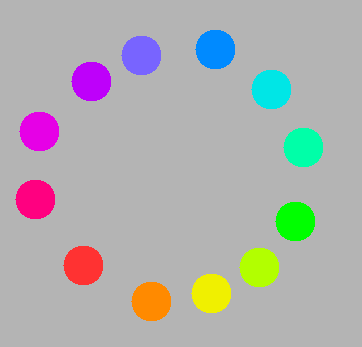
\includegraphics[width=0.7\textwidth]{a2/kreis}}
\caption{Die Abbildung zeigt den von uns erstellten Farbkreis durch die Anordnung der Farbstimuli nach dem oben beschriebenen Prinzip.}
\label{farbkreis}
\end{figure}


\subsection{Farbmischung \rom{1}}
Die ersten drei Farben (Rot, Grün, Blau) sind Grundfarben und konnten einfach durch die Einstellung des entsprechenden Reglers auf $100\%$ hergestellt werden (siehe Abbildungen \ref{rotmix}-\ref{blaumix}).  \\
Gelb wurde durch die Kombination von Rot ($100\%$) und Grün ($100\%$) hergestellt. 
Magenta wurde durch die Kombination von Rot ($100\%$) und Blau ($100\%$) hergestellt. 
Cyan wurde durch die Kombination von Blau ($100\%$) und Grün ($100\%$) hergestellt.  \\
Die Mischung von mittlerem Grau wurde durch die Einstellung der RGB-Werte drei Farben auf $50\%$ erreicht. \\
Schwarz wurde durch die Einstellung auf $0\%$ aller RGB-Werte beobachtet. \\



\makebox[\textwidth][c]{
\begin{minipage}[t]{0.6\textwidth} 
\begin{figure}[H]
\makebox[\textwidth][c]{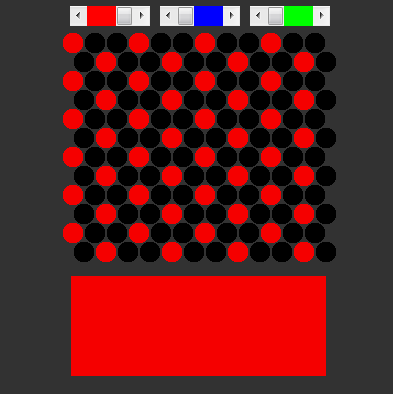
\includegraphics[width=\textwidth]{a3/rot}}
\caption{Hier ist die Herstellung der Farbe \textit{Rot} mittels Farmischung der RGB-Farben zu sehen.}
\label{rotmix}
\end{figure}
\end{minipage} 
\hfill \hspace{1.5cm}
\begin{minipage}[t]{0.6\textwidth} 
\vspace{0pt}
\begin{figure}[H]
\makebox[\textwidth][c]{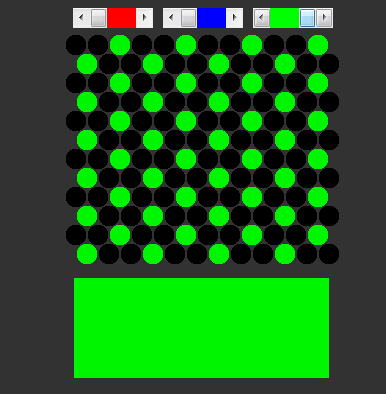
\includegraphics[width=\textwidth]{a3/gruen}}
\caption{Hier ist die Herstellung der Farbe \textit{Grün} mittels Farmischung der RGB-Farben zu sehen.}
\label{gruenmix}
\end{figure}
\end{minipage} }

\makebox[\textwidth][c]{
\begin{minipage}[t]{0.6\textwidth} 
\begin{figure}[H]
\makebox[\textwidth][c]{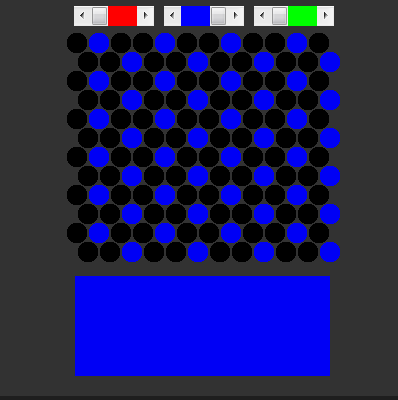
\includegraphics[width=\textwidth]{a3/blau}}
\caption{Hier ist die Herstellung der Farbe \textit{Blau} mittels Farmischung der RGB-Farben zu sehen.}
\label{blaumix}
\end{figure}
\end{minipage} 
\hfill \hspace{1.5cm}
\begin{minipage}[t]{0.6\textwidth} 
\vspace{0pt}
\begin{figure}[H]
\makebox[\textwidth][c]{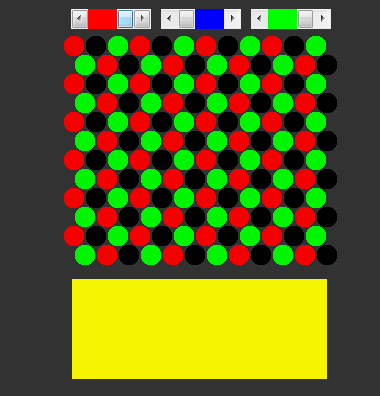
\includegraphics[width=\textwidth]{a3/gelb}}
\caption{Hier ist die Herstellung der Farbe \textit{Gelb} mittels Farmischung der RGB-Farben zu sehen.}
\label{gelbmix}
\end{figure}
\end{minipage} }

\makebox[\textwidth][c]{
\begin{minipage}[t]{0.6\textwidth} 
\begin{figure}[H]
\makebox[\textwidth][c]{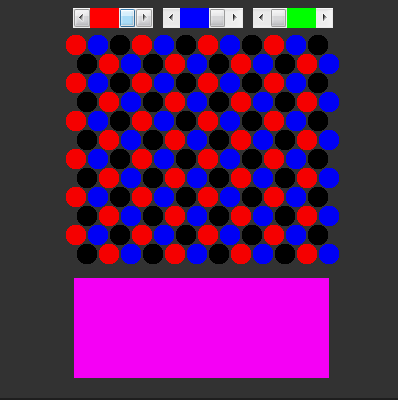
\includegraphics[width=\textwidth]{a3/magenta}}
\caption{Hier ist die Herstellung der Farbe \textit{Rot} mittels Farmischung der RGB-Farben zu sehen.}
\label{magentamax}
\end{figure}
\end{minipage} 
\hfill \hspace{1.5cm}
\begin{minipage}[t]{0.6\textwidth} 
\vspace{0pt}
\begin{figure}[H]
\makebox[\textwidth][c]{\includegraphics[width=\textwidth]{a3/Cyan}}
\caption{Hier ist die Herstellung der Farbe \textit{Grün} mittels Farmischung der RGB-Farben zu sehen.}
\label{cyanmix}
\end{figure}
\end{minipage} }

\makebox[\textwidth][c]{
\begin{minipage}[t]{0.6\textwidth} 
\vspace{0pt}
\begin{figure}[H]
\makebox[\textwidth][c]{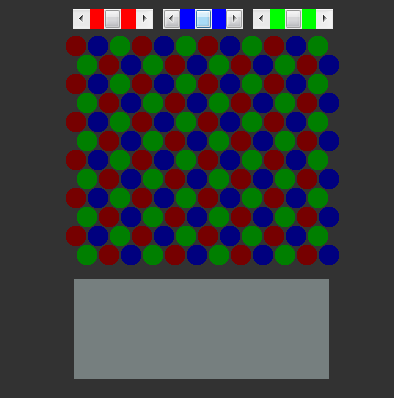
\includegraphics[width=\textwidth]{a3/grau}}
\caption{Hier ist die Herstellung der Farbe \textit{Grau} mittels Farmischung der RGB-Farben zu sehen.}
\label{graumix}
\end{figure}
\end{minipage}
\hfill \hspace{1.5cm}
\begin{minipage}[t]{0.6\textwidth} 
\begin{figure}[H]
\makebox[\textwidth][c]{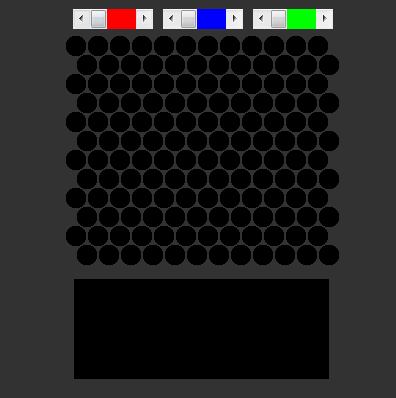
\includegraphics[width=\textwidth]{a3/schwarz}}
\caption{Hier ist die Herstellung der Farbe \textit{Schwarz} mittels Farmischung der RGB-Farben zu sehen.}
\label{schwarzmix}
\end{figure}
\end{minipage}  }
Die verwendete Farbmischung ist hier die additive Farbmischung, da mehrere Lichtstimuli überlagert werden. \\

Dass das mittlere Grau mit einer Einstellung von allen RGB-Werten auf $50\%$ erreicht wurde (\ref{graumix}), ist auf die Normierung der RGB-Werte zurückzuführen. Die Gesamtleuchtdichte für Weiß ergibt sich aus der Überlagerung der Farben Rot, Grün und Blau auf jeweils $100\%$. Außerdem halbiert sich der Helligkeitseindruck jeder Farbe bei Halbierung der RGB-Werte, sodass man mit der mittleren Einstellung einen mittleren Grauton erhält. 


\subsection{Farbintentität}
Der Weißpunkt hat im Yxy-Raum die Koordinaten $(100,0.307,0.347)$ und im L*a*b*-Farbraum die Koordinaten (100,0,0) (siehe Abbildung \ref{weisspunkt}).  \\


\begin{figure}[H]
\makebox[1\textwidth][c]{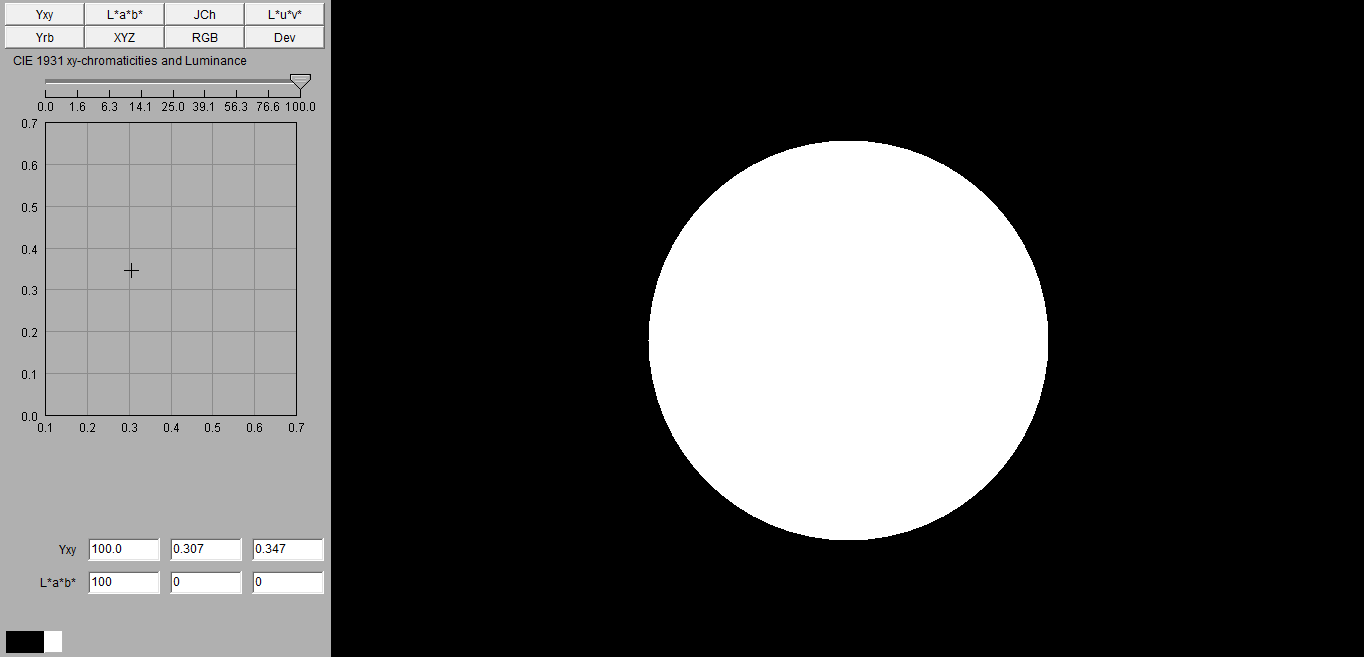
\includegraphics[width=1.3\textwidth]{a4/xyx2}}
\caption{In dem Screenshot ist zu sehen, wo der Weißpunkt im Yxy- und im Farbraum liegt.}
\label{weisspunkt}
\end{figure}

Mit einer Intensität von $6.3$ (siehe \ref{blau1}) ließ sich das Farbdreieck gut im Koordinatensystem erkennen. Das Farbdreieck ist ein Ebenenschnitt aus dem dreidimensionalen Farbenraum, das man durch eine Normierung der Achsen erhält. Hier erfolgt die Normierung für Weiß, sodass sich der Weißpunkt durch eine Veränderung der Intensität nicht verändert. Es repräsentiert das sichtbare Spektrums, d.h. alle Farben der Punkte die im Koordinatensystem (siehe \ref{blau1}) innerhalb des Dreiecks liegen, sind für uns sichtbar. Alle weiteren Punkte, die sich außerhalb des Dreiecks befinden repräsentieren Farben, die wir nicht sehen können. 

\begin{figure}[H]
\makebox[\textwidth][c]{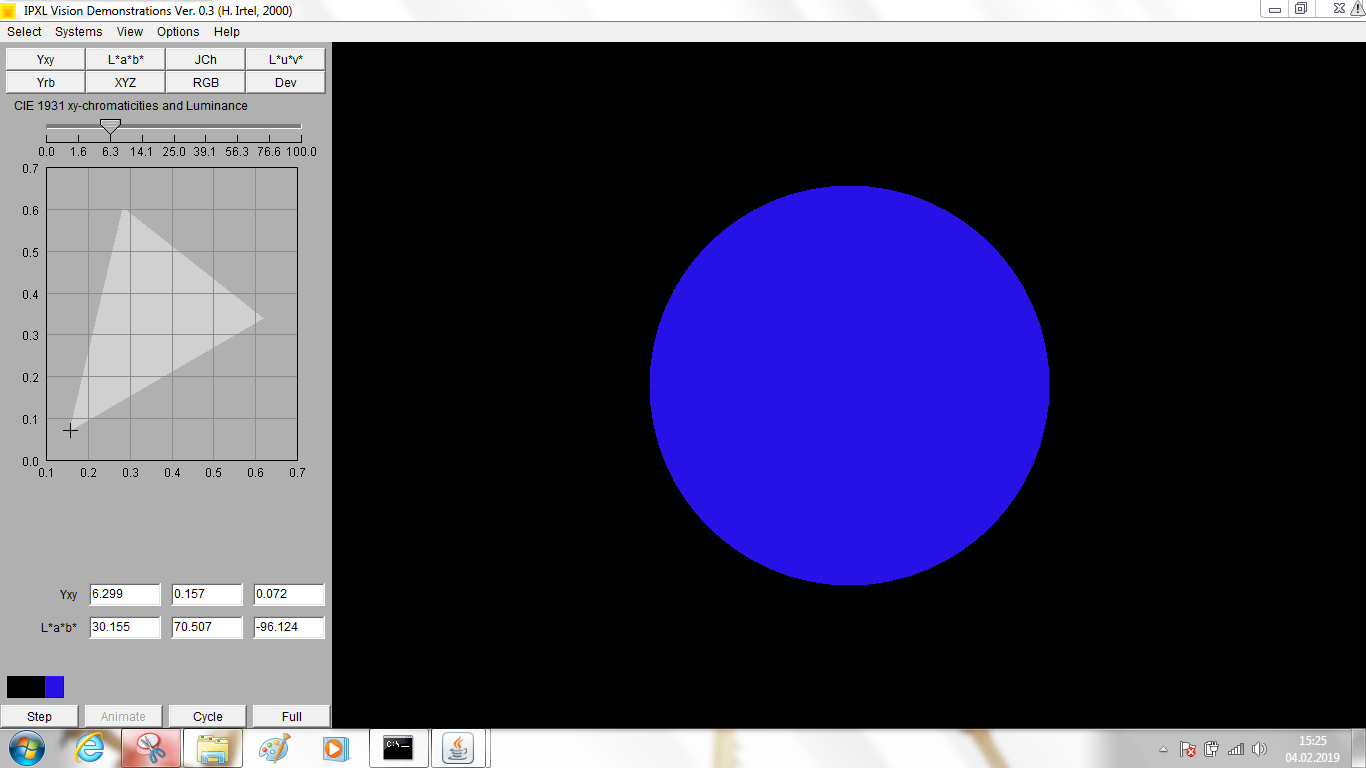
\includegraphics[width=1.3\textwidth]{a4/blau1}}
\caption{Zu sehen ist auf der linken Seite das Koordinatensystem mit dem Farbdreieck bei höchster Intensität, bevor die Fläche nicht mehr dreieckig ist.}
\label{blau1}
\end{figure}

Im Folgenden sind Veränderungen des obigen Blautons (\ref{blau1}) bezüglich der Helligkeit (\ref{blau2}-\ref{blau3}), des Farbtons (\ref{blau4}-\ref{blau5}) und der Sättigung (\ref{blau6}-\ref{blau8}) des Stimulus dokumentiert. \\

Für die Verringerung der Helligkeit wurde der Regler für die Intensität auf verschiedene Werte eingestellt. 

\makebox[\textwidth][c]{
\begin{minipage}[t]{0.6\textwidth} 
\vspace{0pt}
\begin{figure}[H]
\makebox[\textwidth][c]{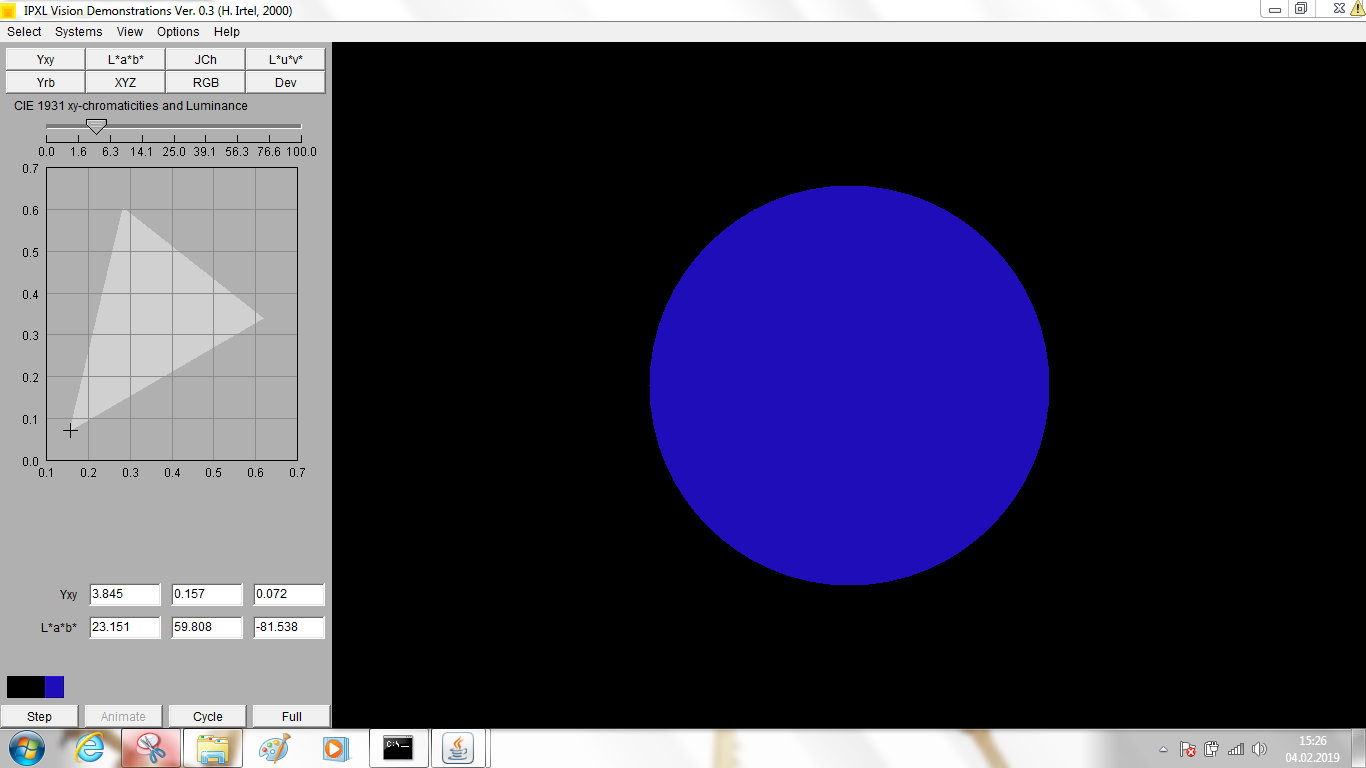
\includegraphics[width=\textwidth]{a4/blau2}}
\caption{Hier ist die Veränderung der Helligkeit (Verringerung) des ursprünglichen Farbtons (siehe oben) zu sehen.}
\label{blau2}
\end{figure}
\end{minipage}
\hfill \hspace{1.5cm}
\begin{minipage}[t]{0.6\textwidth} 
\begin{figure}[H]
\makebox[\textwidth][c]{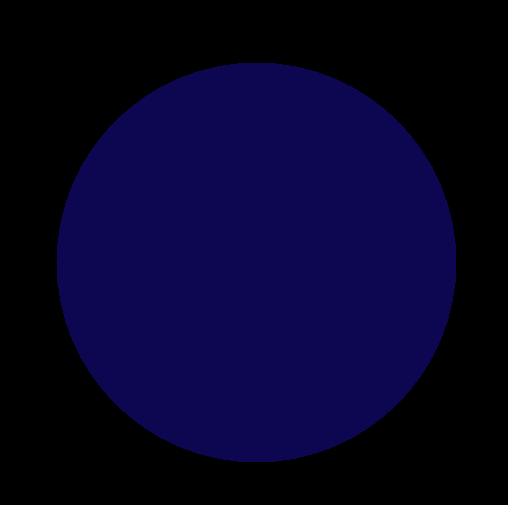
\includegraphics[width=\textwidth]{a4/blau3}}
\caption{Hier ist die weitere Verringerung der Helligkeit des Farbstimulus zu sehen. }
\label{blau3}
\end{figure}
\end{minipage}} \\

Für die Veränderung des Farbtons wurde der Punkt entlang der Seiten des Dreiecks ein Stück verschoben. Ursprünglich lag der Punkt in der unteren Ecke für Blau im Farbdreieck (siehe \ref{blau1}).

\makebox[\textwidth][c]{
\begin{minipage}[t]{0.6\textwidth} 
\vspace{0pt}
\begin{figure}[H]
\makebox[\textwidth][c]{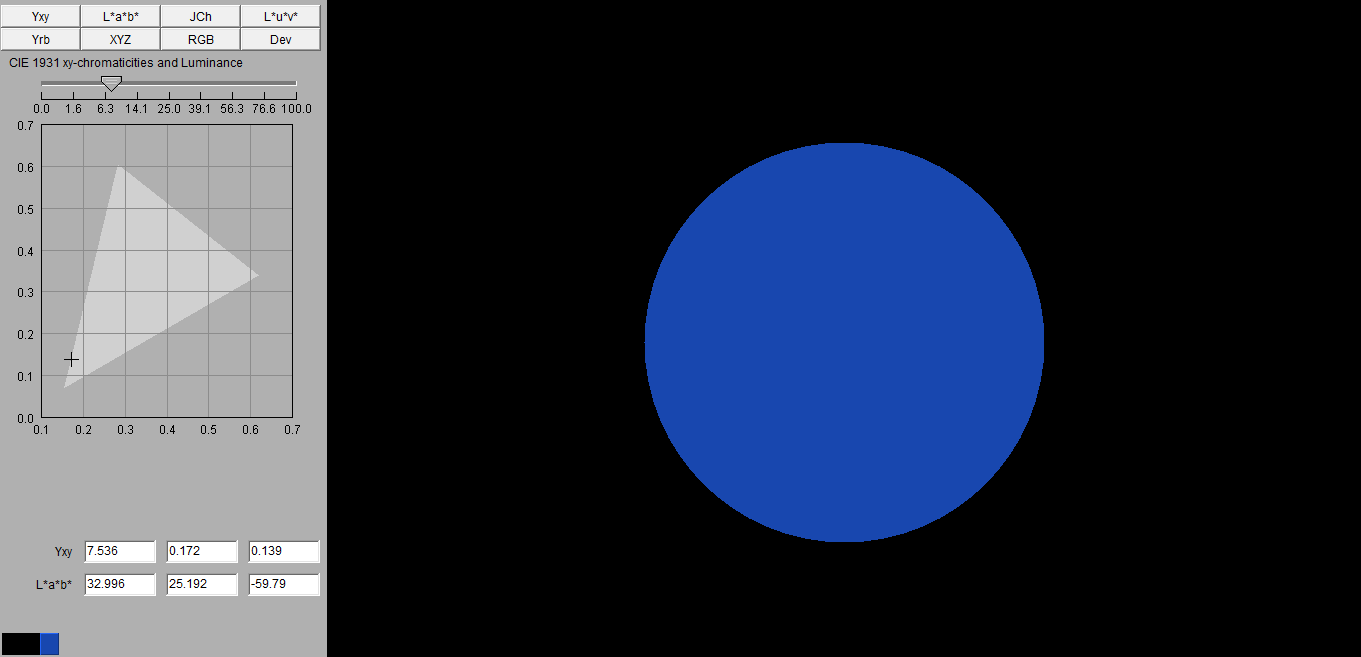
\includegraphics[width=\textwidth]{a4/blau4}}
\caption{In dieser Abbildung zeigt der Farbstimulus eine Veränderung des Farbtons. }
\label{blau4}
\end{figure}
\end{minipage}
\hfill \hspace{1.5cm}
\begin{minipage}[t]{0.6\textwidth} 
\begin{figure}[H]
\makebox[\textwidth][c]{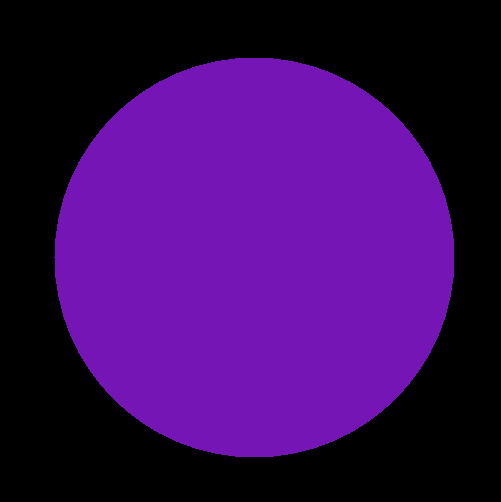
\includegraphics[width=\textwidth]{a4/blau5}}
\caption{In dieser Abbildung zeigt der Farbstimulus eine weitere Veränderung des Farbtons.}
\label{blau5}
\end{figure}
\end{minipage}}

Für die Veränderung der Sättigung wurde der Punkt im Koordinatensystem von der ursprünglichen Farbe (in der Ecke für Blau im Farbdreieck) auf der Geraden zum Weißpunkt verschoben.

\makebox[\textwidth][c]{
\begin{minipage}[t]{0.6\textwidth} 
\vspace{0pt}
\begin{figure}[H]
\makebox[\textwidth][c]{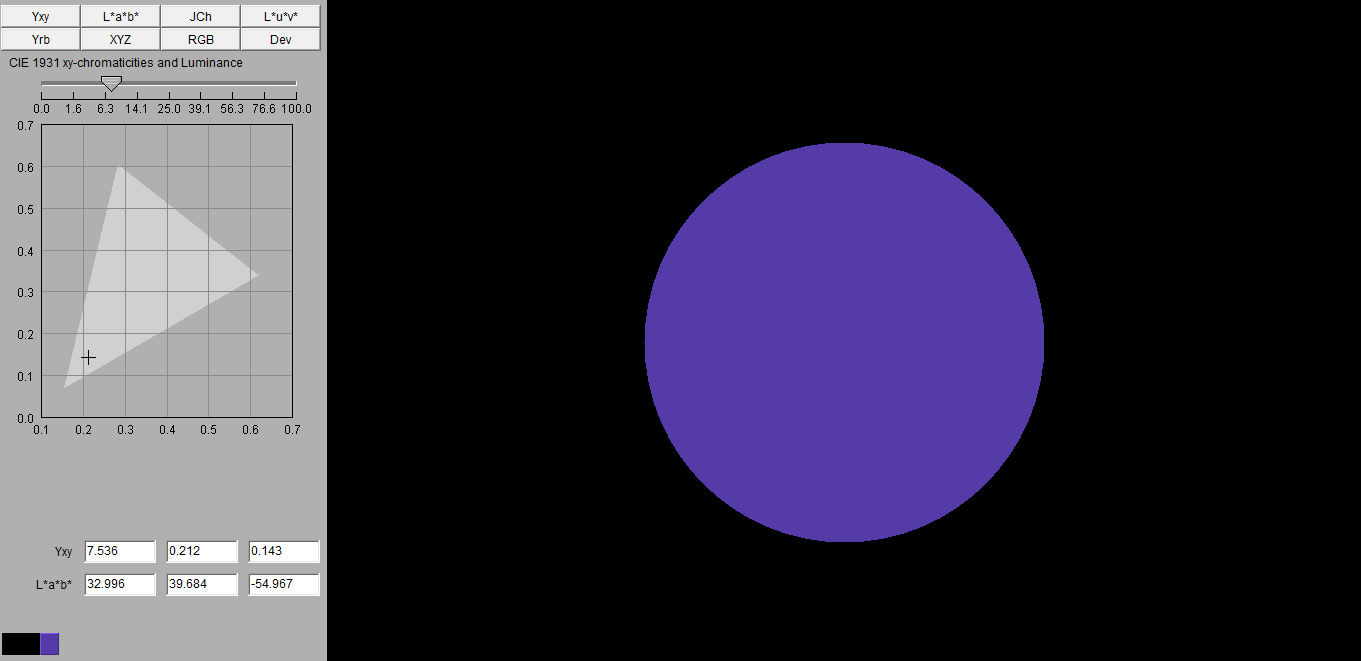
\includegraphics[width=\textwidth]{a4/blau6}}
\caption{Diese Abbildung zeigt die Verringerung der Sättigung des ursprünglichen Blautons (siehe oben).}
\label{blau6}
\end{figure}
\end{minipage}
\hfill \hspace{1.5cm}
\begin{minipage}[t]{0.6\textwidth} 
\begin{figure}[H]
\makebox[\textwidth][c]{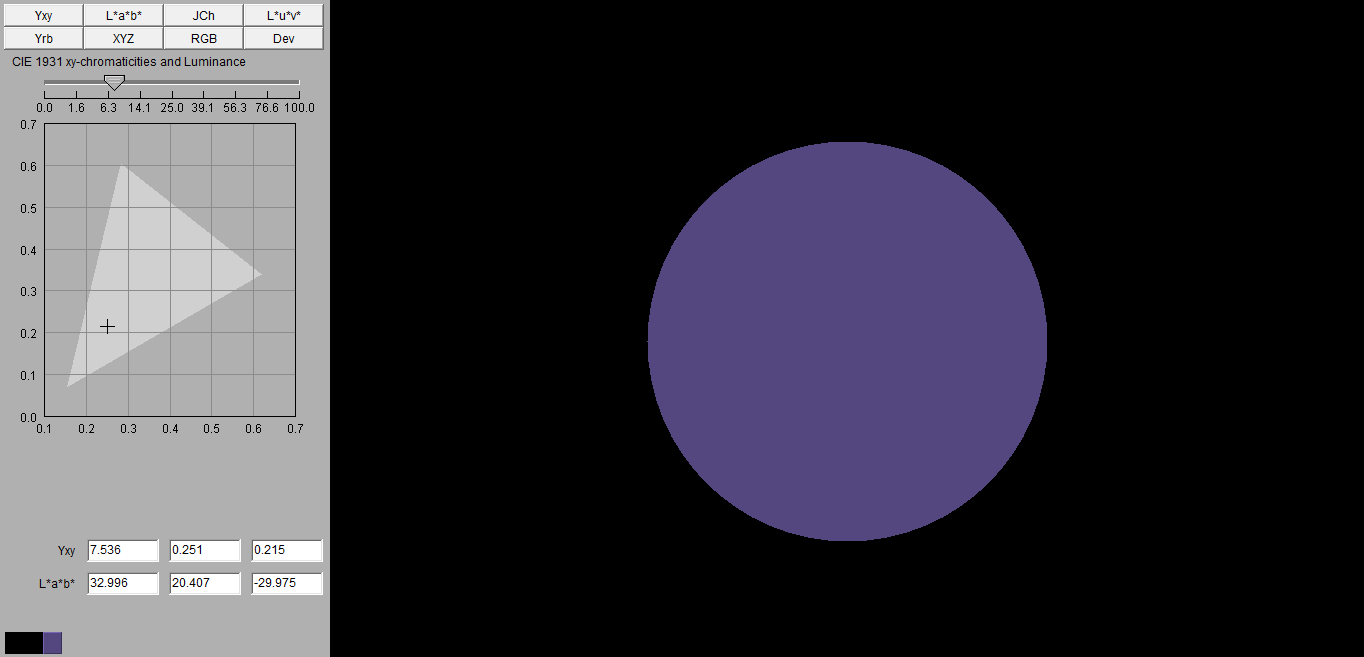
\includegraphics[width=\textwidth]{a4/blau7}}
\caption{Diese Abbildung zeigt eine weitere Verringerung der Sättigung des Farbtons.}
\label{blau7}
\end{figure}
\end{minipage}}

\makebox[\textwidth][c]{
\begin{minipage}[t]{0.6\textwidth} 
\vspace{0pt}
\begin{figure}[H]
\makebox[\textwidth][c]{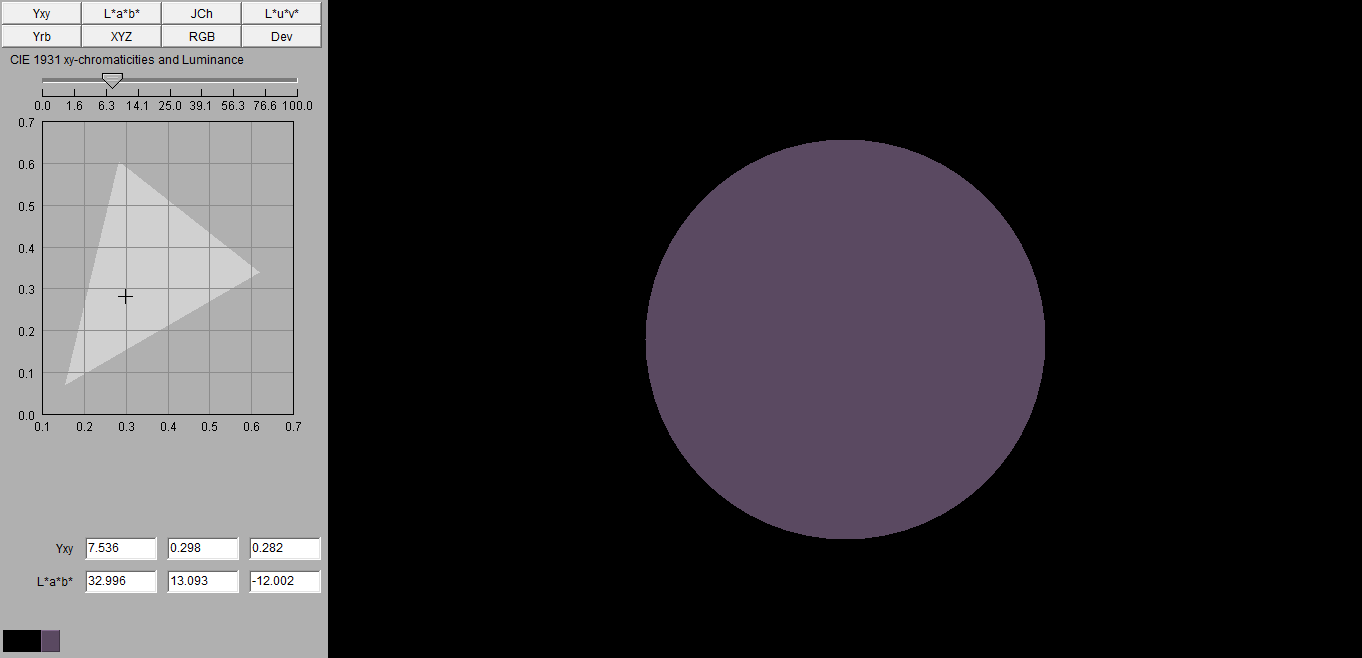
\includegraphics[width=\textwidth]{a4/blau8}}
\caption{Diese Abbildung zeigt eine weitere Verringerung der Sättigung des Farbtons.}
\label{blau8}
\end{figure}
\end{minipage}} \\

Wird die Sättigung bei konstanter Intensität verändert (siehe \ref{blau6}-\ref{blau8}), wird der subjektiv wahrgenommene Effekt der Farbe schwächer, sie wirkt dunkler, obwohl die Helligkeit nicht verändert wurde. \\

Bei Veränderung der Intensität des Stimulus (siehe \ref{blau1}-\ref{blau3}) wirkt die Farbe bei höherer Intensität leuchtender und heller, während sie bei niedriger Intensität dunkler wird. \\

Im Folgenden wurde die Hintergrundfarbe des Stimulus variiert.

\makebox[\textwidth][c]{
\begin{minipage}[t]{0.6\textwidth} 
\vspace{0pt}
\begin{figure}[H]
\makebox[\textwidth][c]{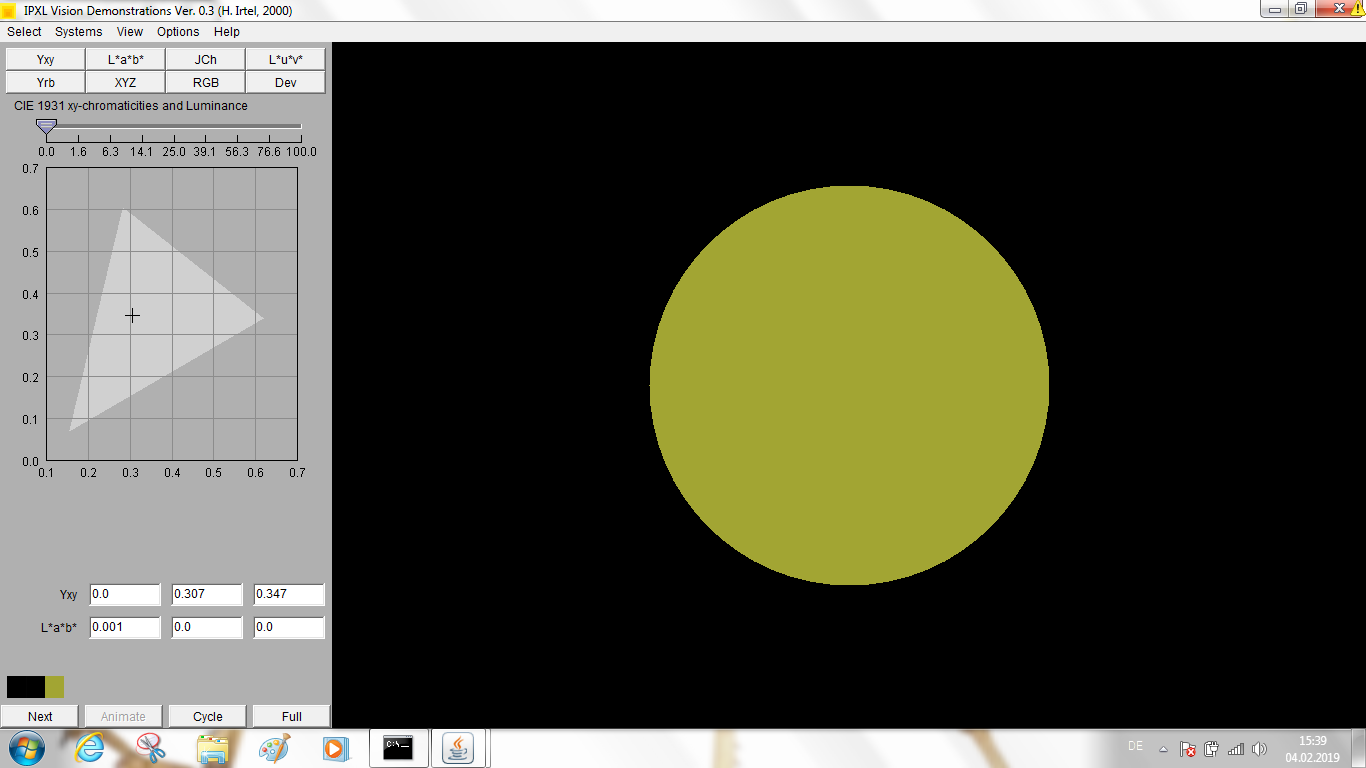
\includegraphics[width=\textwidth]{a4/hintergrund1}}
\caption{Hier ist der Farbstimulus mit einem schwarzen Hintergrund gezeigt.}
\label{hintergrund1}
\end{figure}
\end{minipage}
\hfill \hspace{1.5cm}
\begin{minipage}[t]{0.6\textwidth} 
\begin{figure}[H]
\makebox[\textwidth][c]{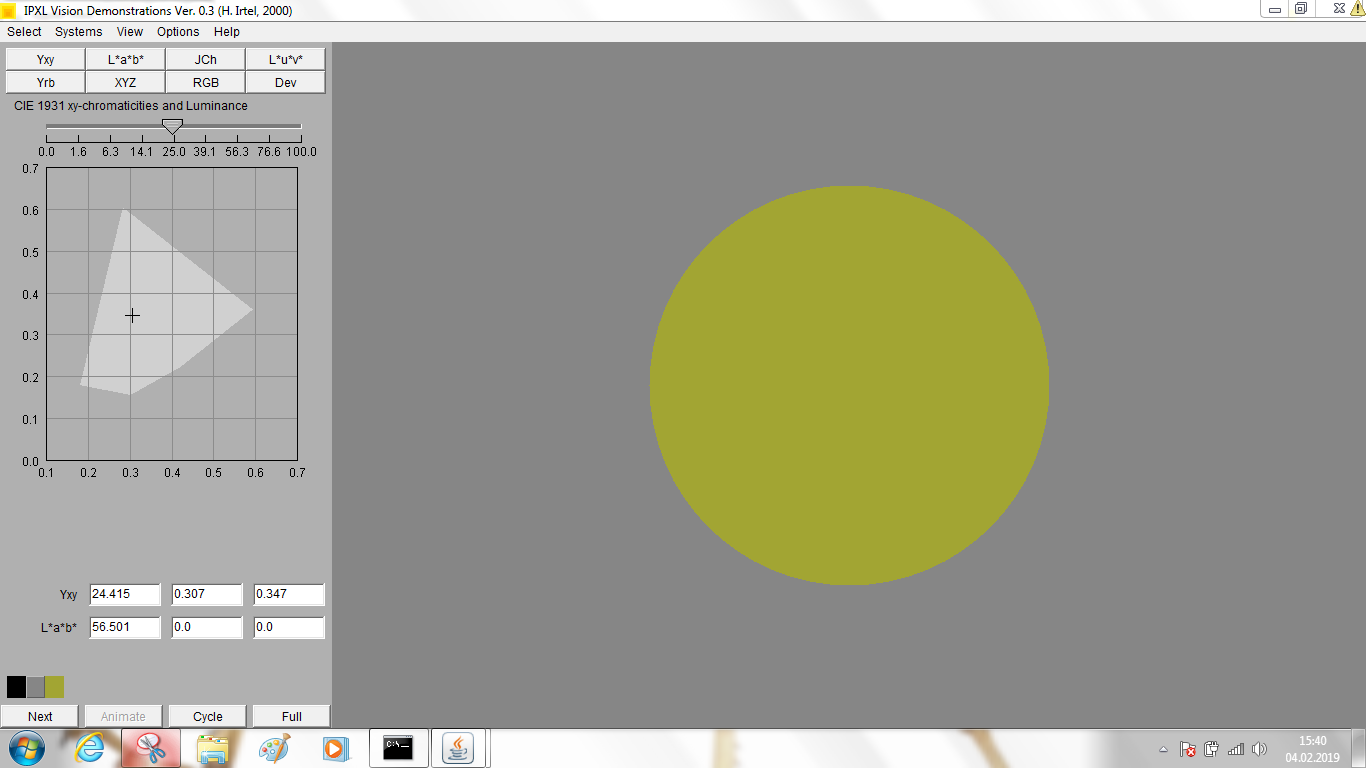
\includegraphics[width=\textwidth]{a4/hintergrund2}}
\caption{Hier ist der Farbstimulus mit einem grauen Hintergrund gezeigt.}
\label{hintergrund2}
\end{figure}
\end{minipage}}

\makebox[\textwidth][c]{
\begin{minipage}[t]{0.6\textwidth} 
\vspace{0pt}
\begin{figure}[H]
\makebox[\textwidth][c]{
\includegraphics[width=\textwidth]{a4/hintergrund3}}
\caption{Hier ist der Farbstimulus mit einem weißen Hintergrund gezeigt.}
\label{hintergrund3}
\end{figure}
\end{minipage}}\\

Im Folgenden wurde die Größe des Farbstimulus verkleinert und erneut die Hintergrundfarbe variiert. \\

\makebox[\textwidth][c]{
\begin{minipage}[t]{0.6\textwidth} 
\vspace{0pt}
\begin{figure}[H]
\makebox[\textwidth][c]{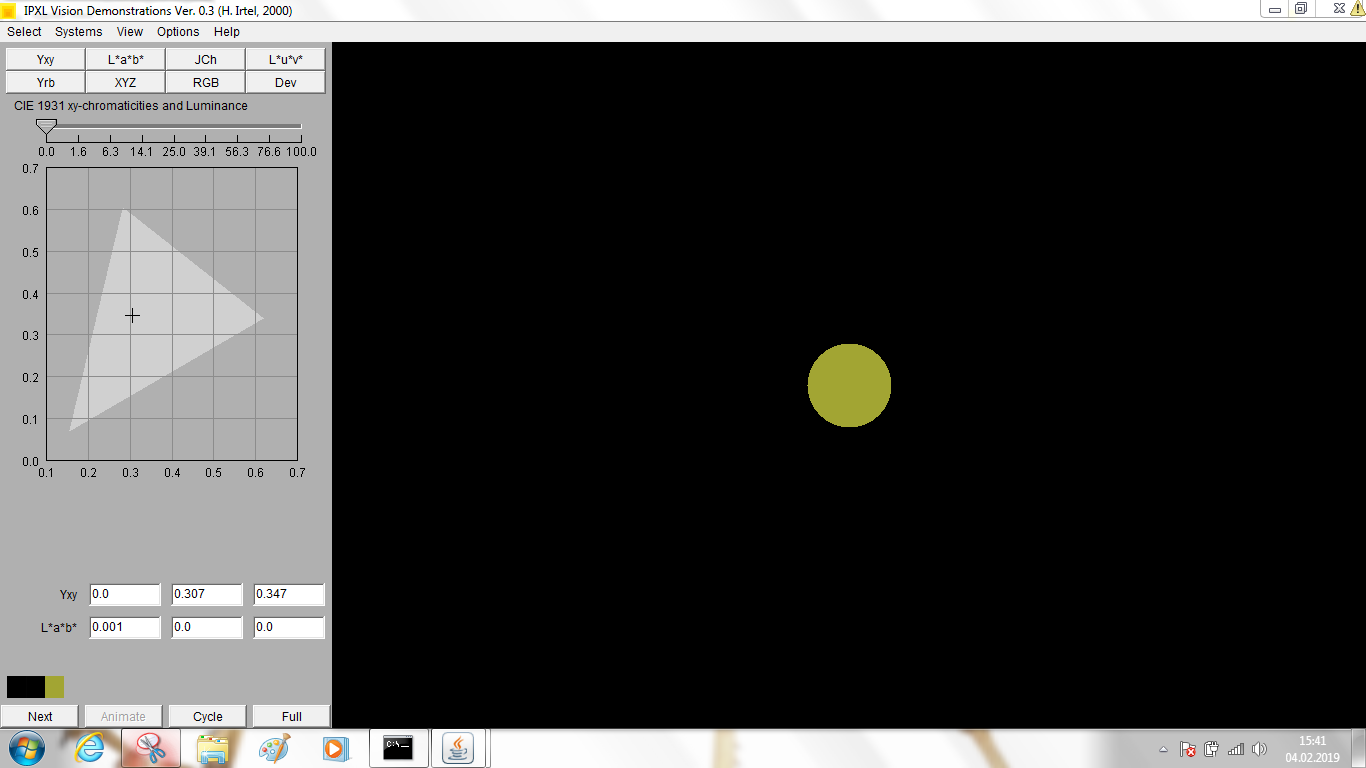
\includegraphics[width=\textwidth]{a4/hintergrund4}}
\caption{Hier ist der kleinere Farbstimulus mit einem schwarzen Hintergrund gezeigt.}
\label{hintergrund3}
\end{figure}
\end{minipage}
\hfill \hspace{1.5cm}
\begin{minipage}[t]{0.6\textwidth} 
\begin{figure}[H]
\makebox[\textwidth][c]{
\includegraphics[width=\textwidth]{a4/hintergrund5}}
\caption{Hier ist der kleinere Farbstimulus mit einem grauen Hintergrund gezeigt.}
\label{hintergrund5}
\end{figure}
\end{minipage}}

\makebox[\textwidth][c]{
\begin{minipage}[t]{0.6\textwidth} 
\vspace{0pt}
\begin{figure}[H]
\makebox[\textwidth][c]{
\includegraphics[width=\textwidth]{a4/hintergrund6}}
\caption{Hier ist der kleinere Farbstimulus mit einem weißen Hintergrund gezeigt.}
\label{hintergrund6}
\end{figure}
\end{minipage}}\\

Es ist zu beobachten, dass der Farbstimulus generell mit einem schwarzen Hintergrund intensiver wird. \\
Außerdem ist bei Betrachtung der Abbildungen mit dem kleineren Farbstimulus zu sehen, dass sich die subjektive Intensität durch die Verkleinerung des Stimulus verringert. 


\subsection{Farbenreihe}
Um die Farbreihe zu erhalten, in der nur der Farbton geändert werden soll, aber die Sättigung und Helligkeit gleich bleiben sollen, haben wir Punkte auf einem imaginären Kreis um den Weißpunkt gewählt. Denn die Sättigung wird über die Entfernung zum Weißpunkt definiert, sodass alle Punkte den gleichen Abstand zu ihm haben müssen, folglich liegen sie auf einem Kreis. (siehe Abbildung \ref{farbton_reihe})
\begin{figure}[H]
\makebox[1\textwidth][c]{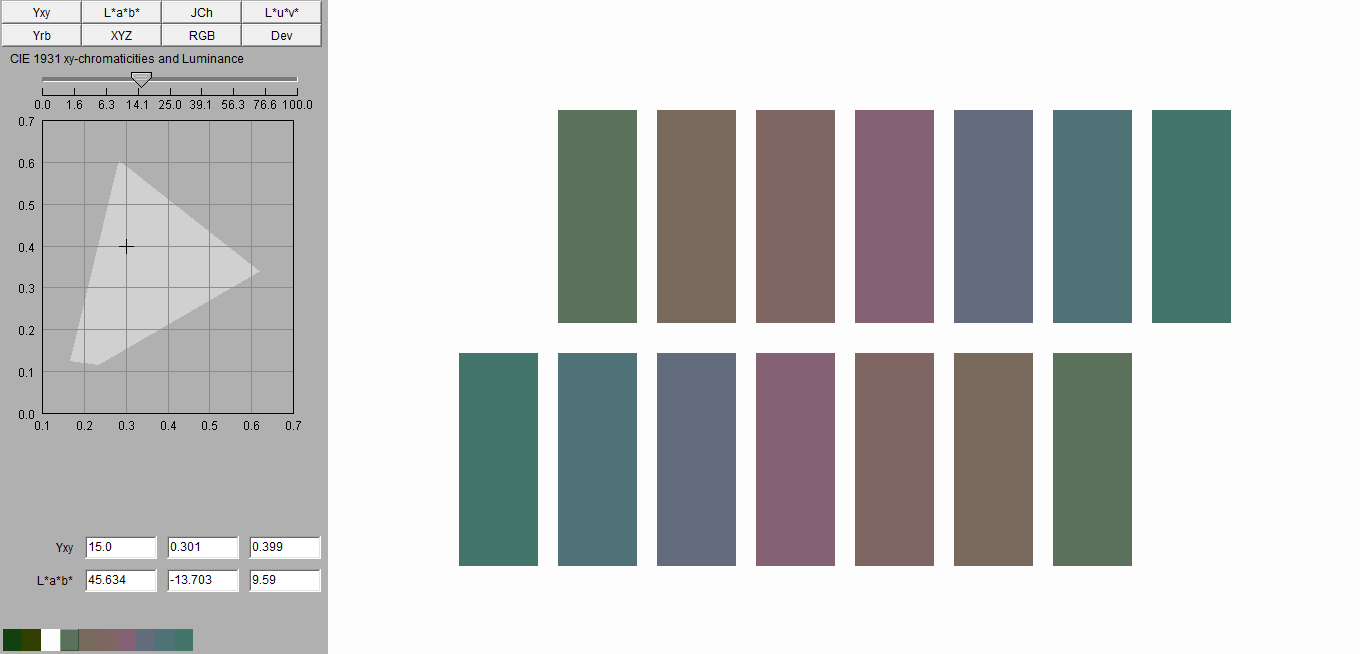
\includegraphics[width=1.3\textwidth]{a5/farbton}}
\caption{Hier ist die Farbreihe mit Änderung des Farbtons zu sehen (Sättigung und Helligkeit konstant).}
\label{farbton_reihe}
\end{figure}


Die Farbreihe mit Variabilität der Helligkeit bei Konstanz der anderen Werte wurde einfach durch die Änderung der Y Koordinate (Intensität) erzeugt. Angefangen bei einem Wert von $80$ links haben wir die Helligkeit sukzessive um $10$ verringert nach rechts (bezogen auf die obere Reihe).  (siehe Abbildung \ref{helligkeit_reihe})
\begin{figure}[H]
\makebox[1\textwidth][c]{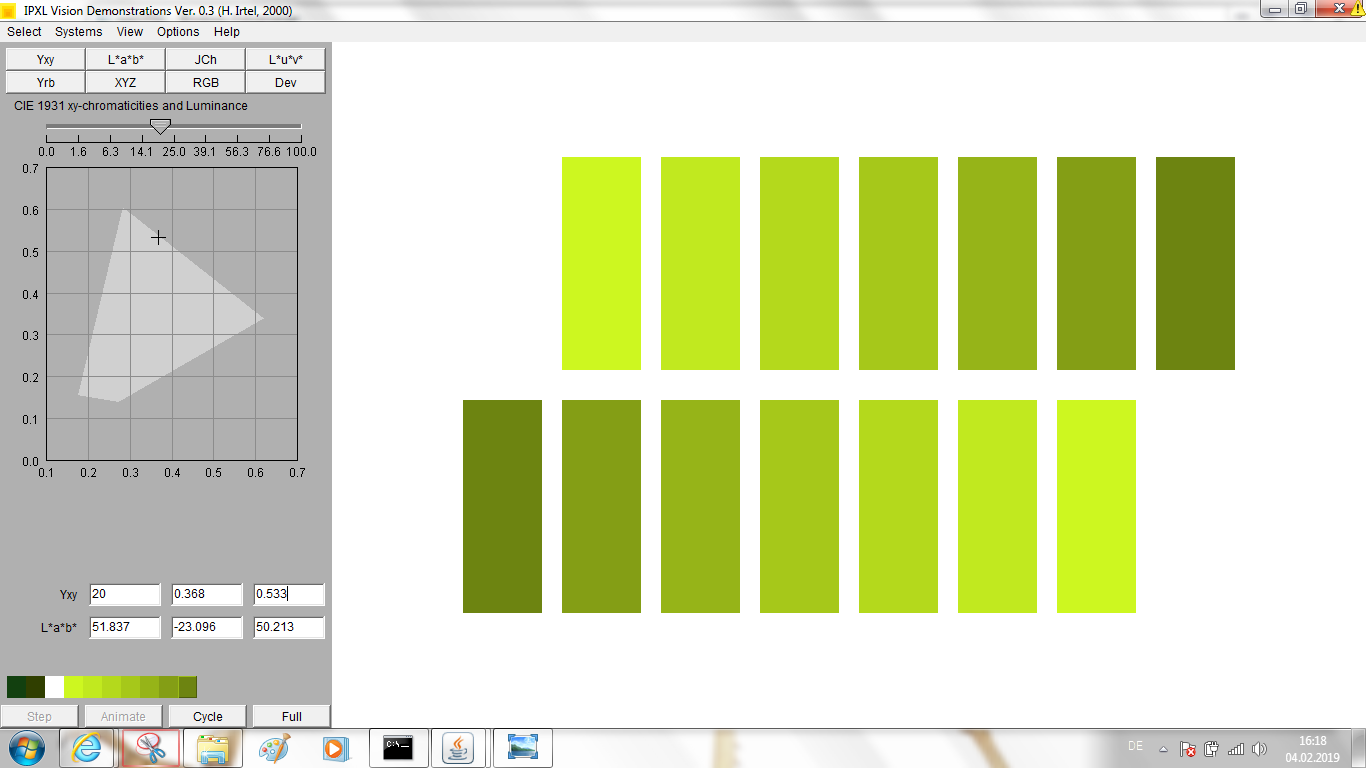
\includegraphics[width=1.3\textwidth]{a5/helligkeit2}}
\caption{Hier ist die Farbreihe mit Änderung der Helligkeit zu sehen (Sättigung und Farbton konstant).}
\label{helligkeit_reihe}
\end{figure}

Die letzte Farbreihe mit Änderungen der Sättigung bei gleichbleibendem Farbton und gleicher Helligkeit haben wir erzeugt, indem wir ausgehend von dem Farbpunkt für Grün in der Ecke des Farbdreiecks (bei Helligkeit $7$) Punkte auf der Geraden zum Weißpunkt gewählt haben. (siehe Abbildung \ref{saettigung_reihe})
\begin{figure}[H]
\makebox[1\textwidth][c]{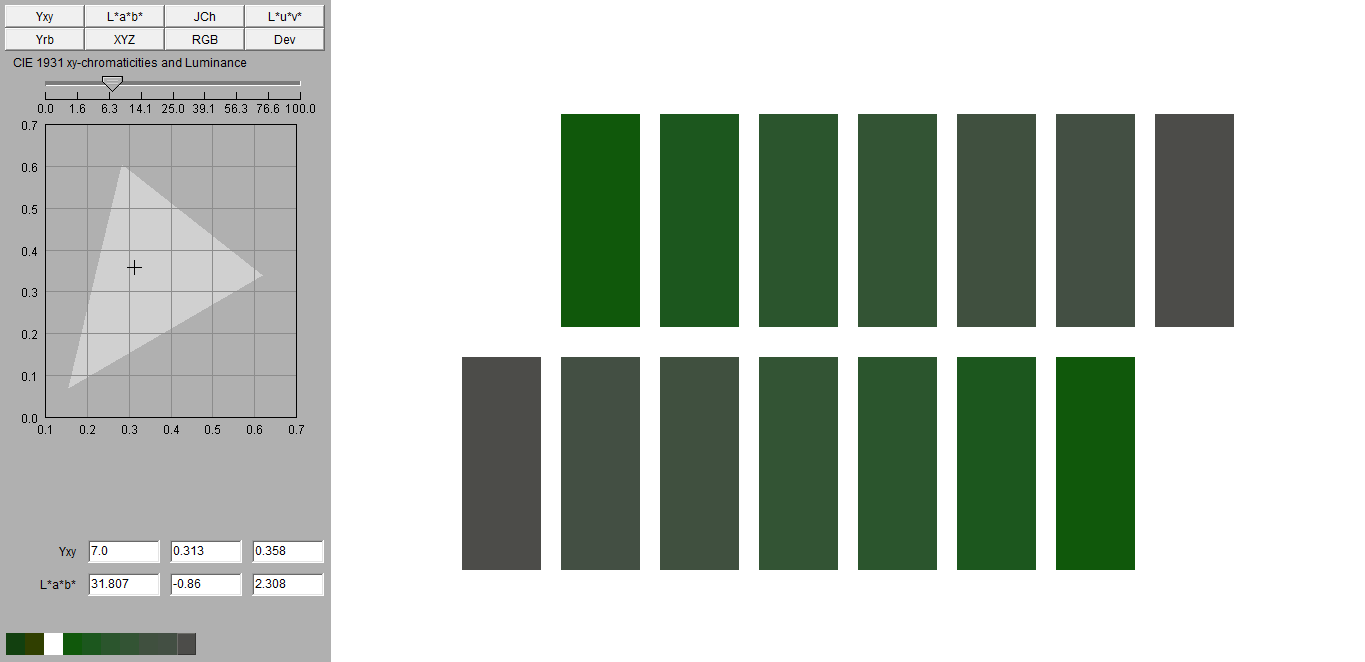
\includegraphics[width=1.3\textwidth]{a5/saettigung}}
\caption{Hier ist die Farbreihe mit Änderung des Sättigung zu sehen (Farbton und Helligkeit konstant).}
\label{saettigung_reihe}
\end{figure}

\subsection{Farbmischung \rom{2}}
Für die linke Fläche haben wir die Farbe mit dem Yxy-Koordinaten $(20,0.3,0.3)$ gewählt. \\
Um im rechten Fenster einen möglichst ähnlichen Farbton nachzumischen haben wir die Farben mit den Koordinaten $(20,0.258, 0.511)$ (grünlich) und $(20,0.325, 0.191)$ (pink) gewählt. 


\begin{figure}[H]
\makebox[1\textwidth][c]{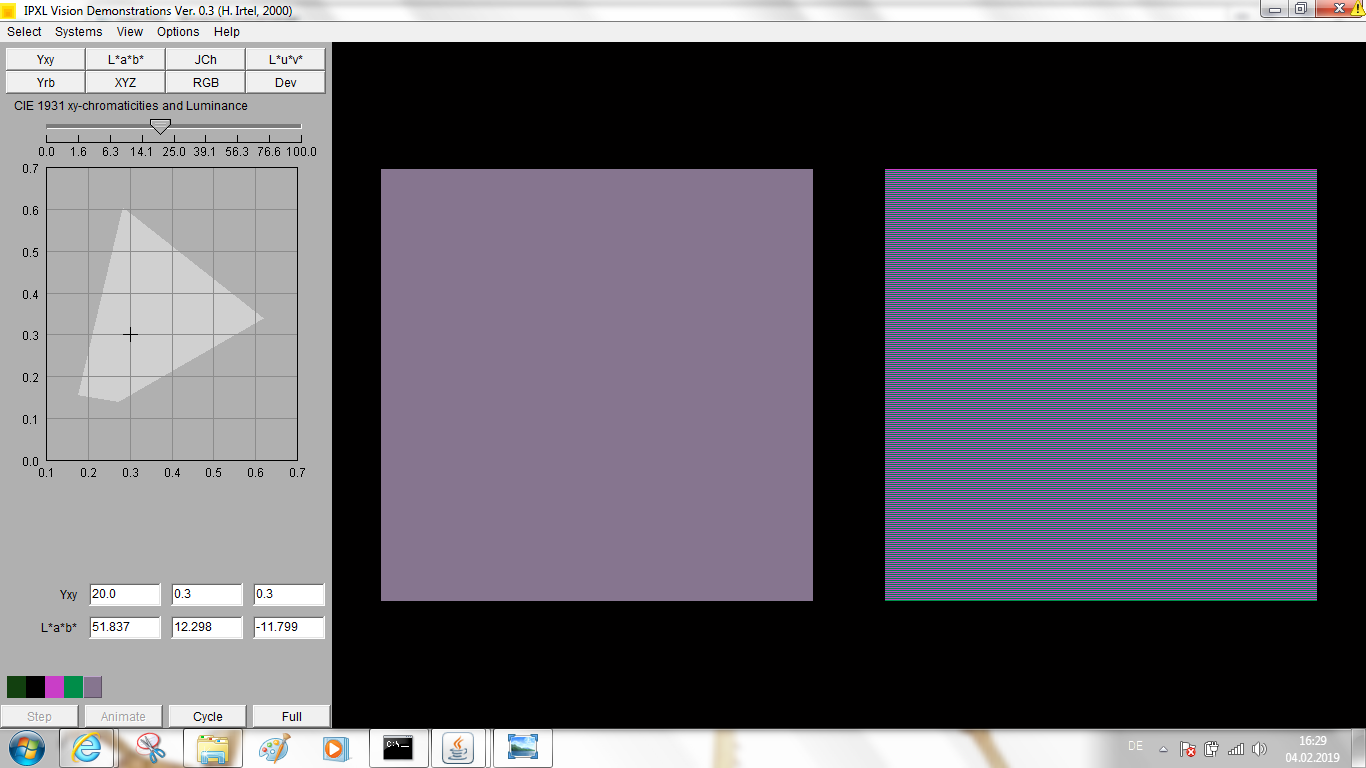
\includegraphics[width=1.3\textwidth]{a6/meta1}}
\caption{Zu sehen ist die Nachmischung der Musterfarbe (links) mit dem ersten Farbpaar (rechts) aus grün und pink.}
\label{meta1}
\end{figure}


Das zweite Farbpaar, mit dem wir die Farbe im linken Fenster nachgemischt haben, hatte die Koordinaten $(20,0.523, 0.392)$ (beige) und $(20,0.184, 0.196)$ (blau). 

\begin{figure}[H]
\makebox[1\textwidth][c]{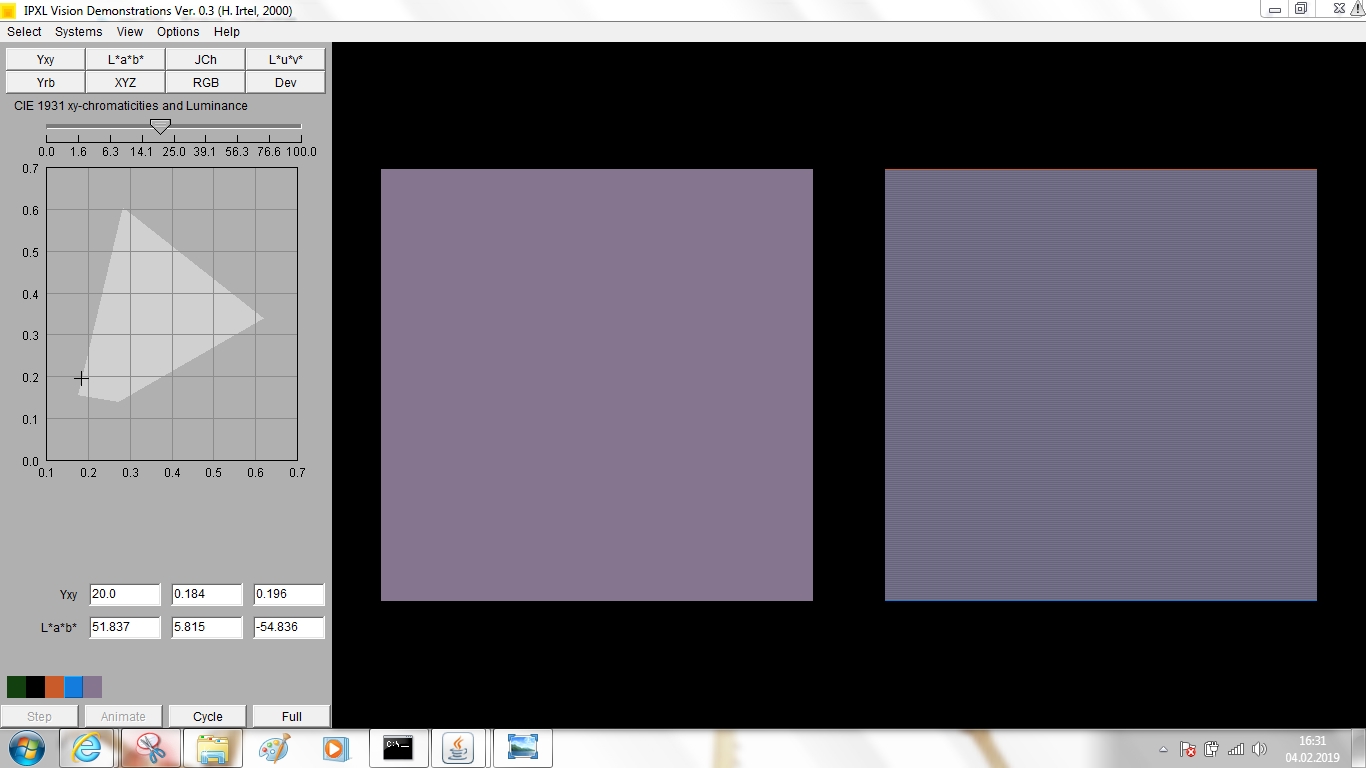
\includegraphics[width=1.3\textwidth]{a6/meta2}}
\caption{Zu sehen ist die Nachmischung der Musterfarbe (links) mit dem zweiten Farbpaar (rechts) aus beige und blau.}
\label{meta2}
\end{figure}

Es ist zu beobachten, dass der Farbort der Mischfarbe sich auf einer Gerade zwischen den Punkten der Einzelfarben befindet. Dies trifft bei beiden verwendeten Farbpaaren zu. \\

In diesem Fall handelt es sich wieder um additive Farbmischung. 

\subsection{Simultaner Farbkontrast}
Der simultane Farbkontrast wird besonders deutlich, wenn man für die äußere, große Fläche einmal eine sehr helle und bei der anderen Fläche eine sehr dunkle Farbe wählt. Außerdem sollten die inneren Flächen auch eher einen hellen Farbton haben. 

\begin{figure}[H]
\makebox[1\textwidth][c]{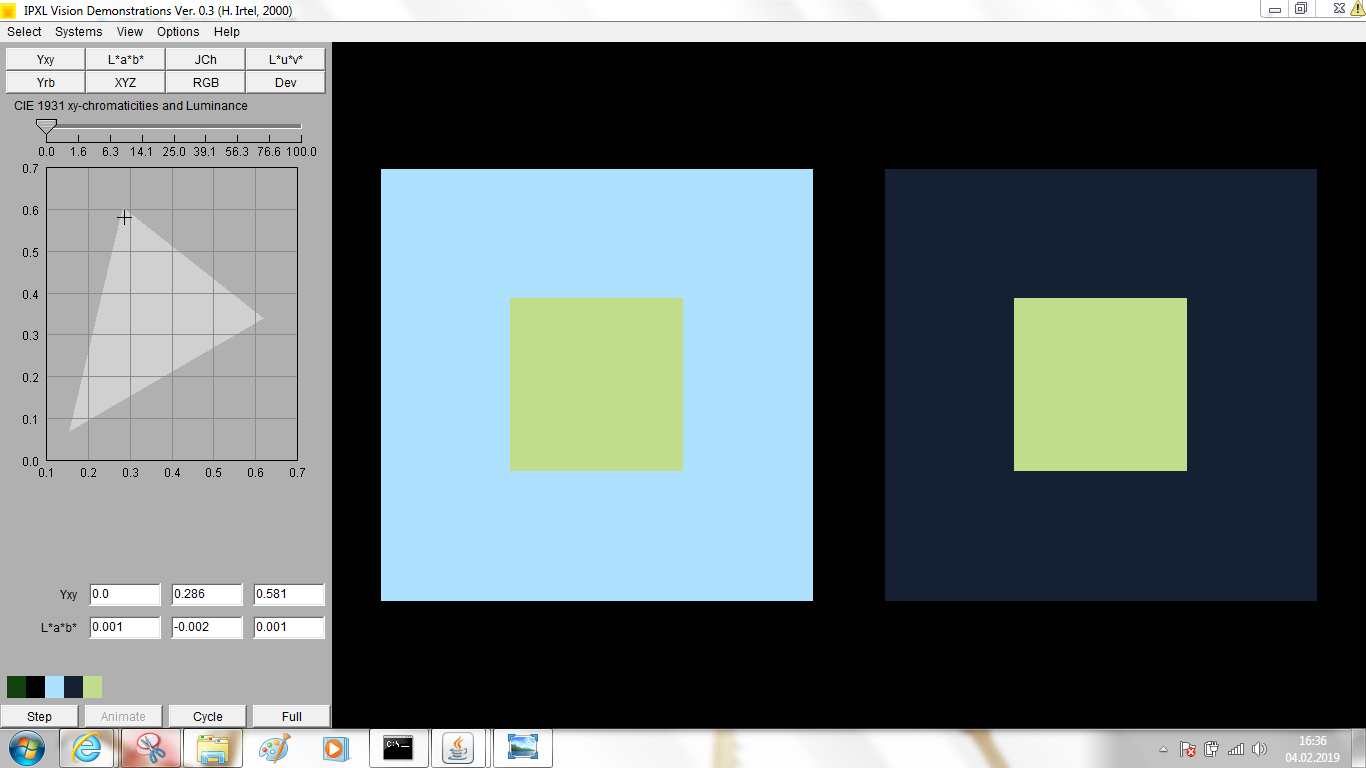
\includegraphics[width=1.3\textwidth]{a7/kontrast}}
\caption{Hier ist die Kombination von unseren ausgewählten Farben für die Simulation des simultanen Farbkonstrastes zu sehen. Links erscheint das innere Quadrat durch die hellere Umgebung dunkler als in der rechten, dunklen Fläche. Außerdem wirken die Übergänge links verschwommener, als beim starken Kontrast auf der rechten Seite.}
\label{meta2}
\end{figure}

\subsection{Sukzessiver Farbkontrast}
In diesem letzten Teil der Versuchsreihe zu Farbensehen ging es um so genannte "{}Nachbilder"{}. Diese entstehen nach intensiver Betrachtung von Reizen. Hier betrachteten wir farbige Reize, also Farbflächen in dem wir 30-60 Sekunden die Mitte der Bilder fokussierten und anschließend ohne die Augen abzuwenden das nächste Bild hervorriefen.

\begin{figure}[H]
\makebox[0.5\textwidth][c]{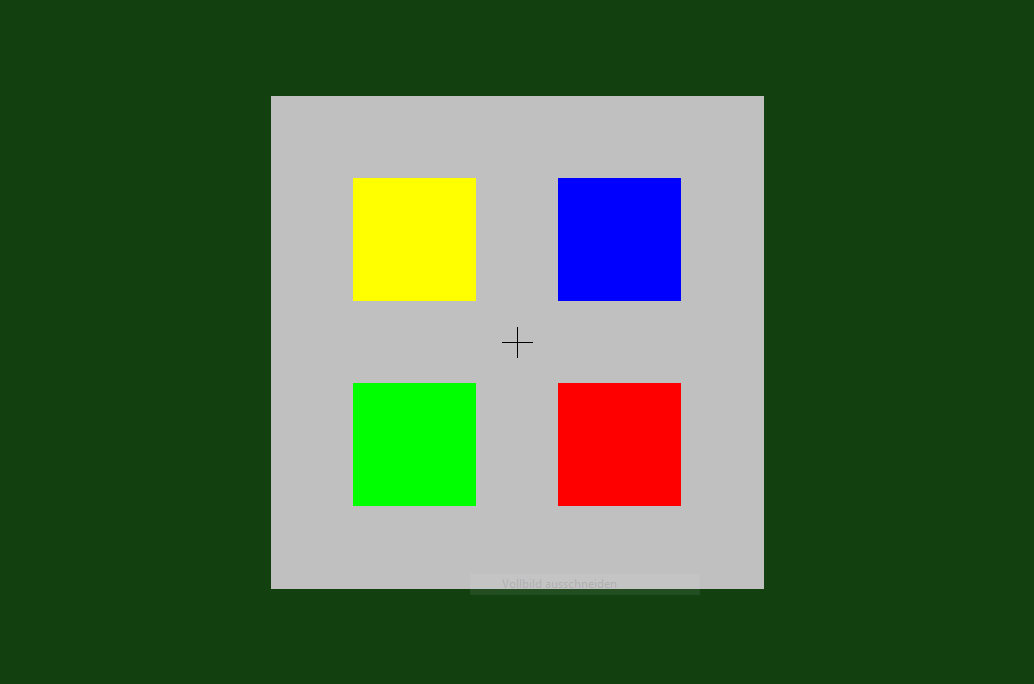
\includegraphics[width=0.5\textwidth]{a8/4farben}}
\makebox[0.5\textwidth][c]{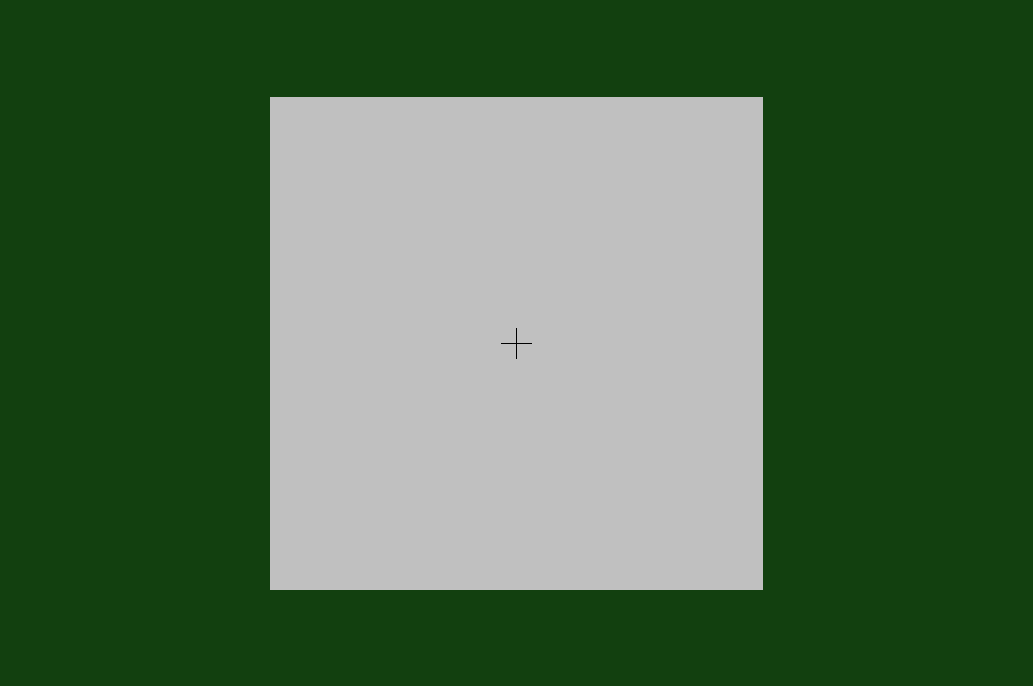
\includegraphics[width=0.5\textwidth]{a8/4farben2}}
\caption{In der Abbildung sind die Bilder aus \textit{Adaption Effects} zu sehen. Im ersten Schritt (links) befinden sich auf dem grauen Hintergrund vier Quadrate in den Farben gelb, blau, grün und rot. Im zweiten Schritt (rechts) sind die farbigen Quadrate verschwunden, lediglich der graue Hintergrund bleibt.}
\label{4farben}
\end{figure}

In Abbildung \ref{4farben} entsteht ein Nachbild, welches jeweils die Quadrate aus dem ersten Bild in komplementärer Färbung darstellt. So scheint sich auf dem lediglich grauen Hintergrund links oben ein blaues, rechts oben ein gelbes, links unten ein rotes und recht unten ein grünes Quadrat zu befinden (siehe Abb. \ref{4farben_nb}). 

\begin{figure}[H]
\makebox[\textwidth][c]{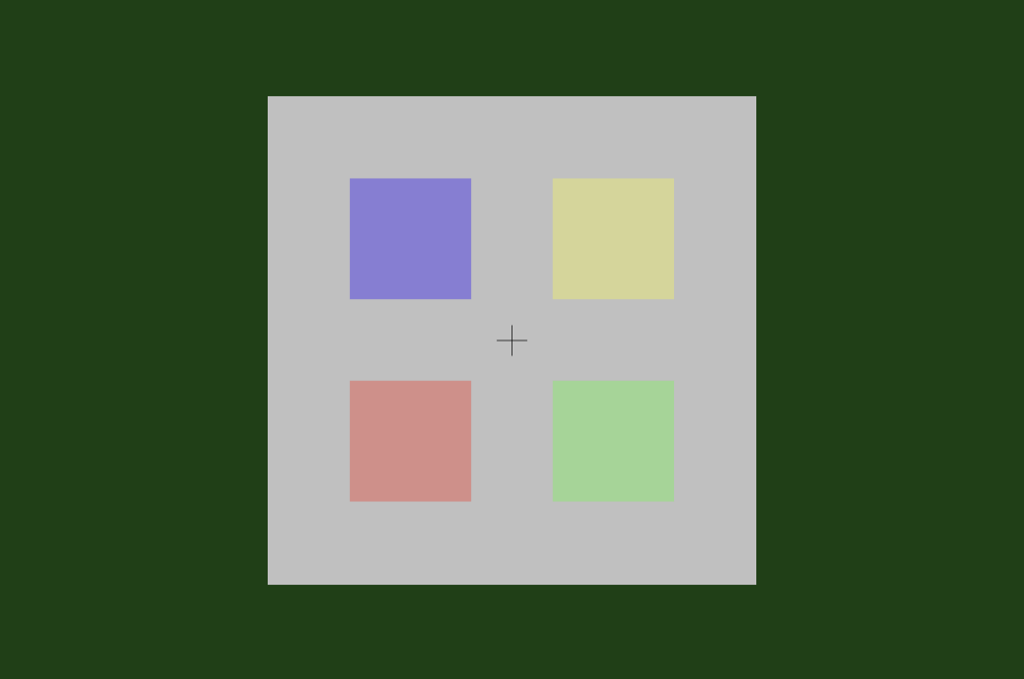
\includegraphics[width=0.5\textwidth]{a8/4farben_nb}}
\caption{Die Abbildung zeigt nachgestellt das gesehene Nachbild von \textit{Adaption Effects}}
\label{4farben_nb}
\end{figure}

\begin{figure}[H]
\makebox[0.5\textwidth][c]{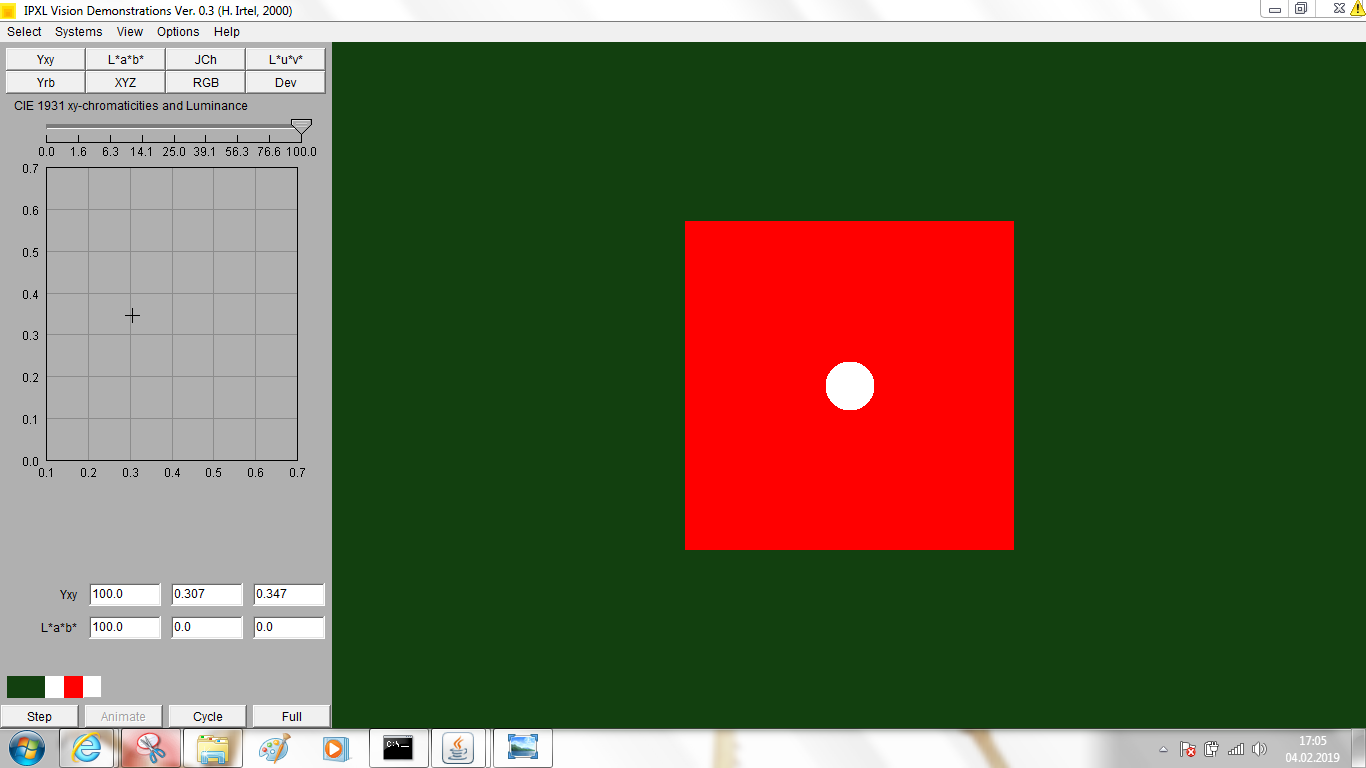
\includegraphics[width=0.5\textwidth]{a8/induction}}
\makebox[0.5\textwidth][c]{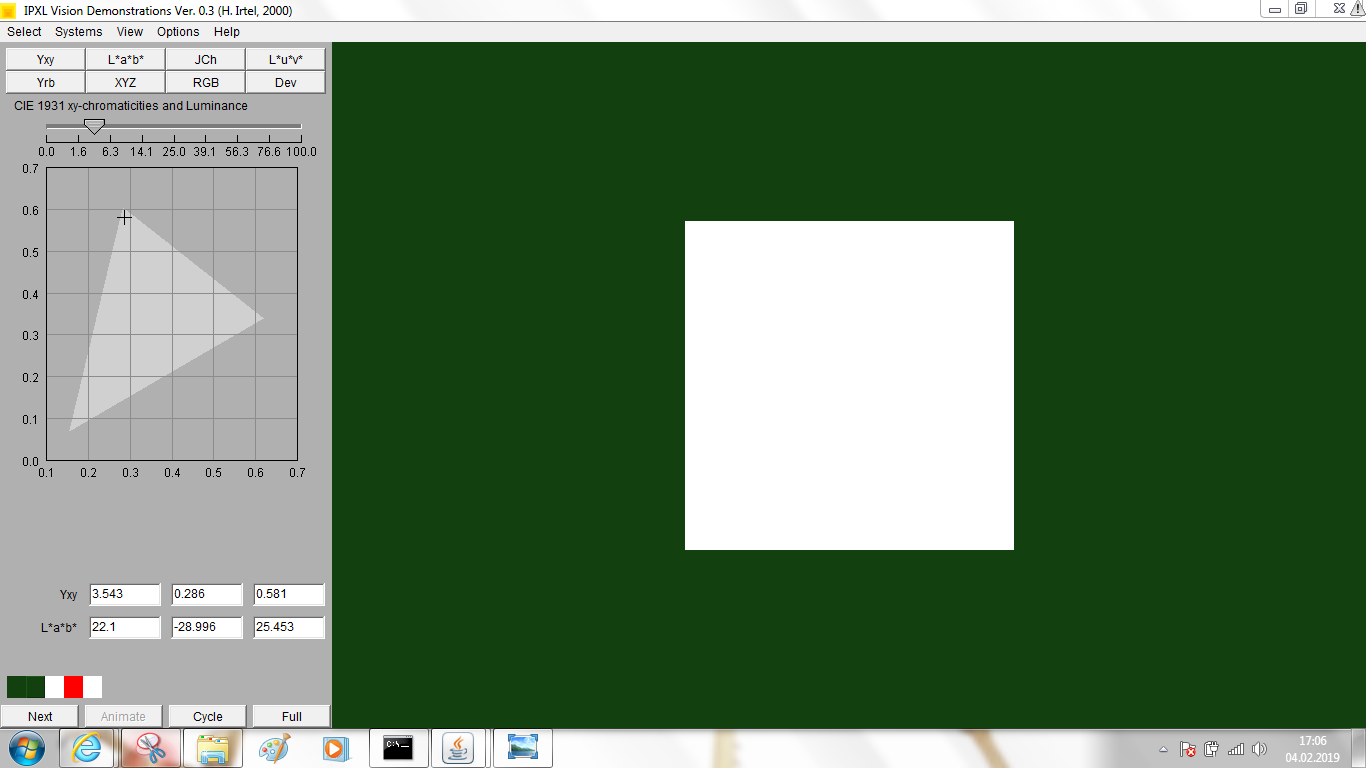
\includegraphics[width=0.5\textwidth]{a8/induction2}}
\caption{Abgebildet sind die Bilder \textit{Induction} zu sehen. Zuerst (links) ist ein roter Hintergrund mit einem weißem Kreis in der Mitte zu sehen. Im Anschluss (rechts) ist die zu betrachtendeFläche weiß.}
\label{induction}
\end{figure}

Nach dem gleichen Konzept wie in Abbildung \ref{4farben} scheint auch das Nachbild in Abbildung \ref{induction}, allerdings erscheint hier nicht nur die ehemals rote Fläche grün, sondern zusätzlich der ehemals weiße Kreis rot (siehe Abb. \ref{induction_nb}.\\

\begin{figure}[H]
\makebox[\textwidth][c]{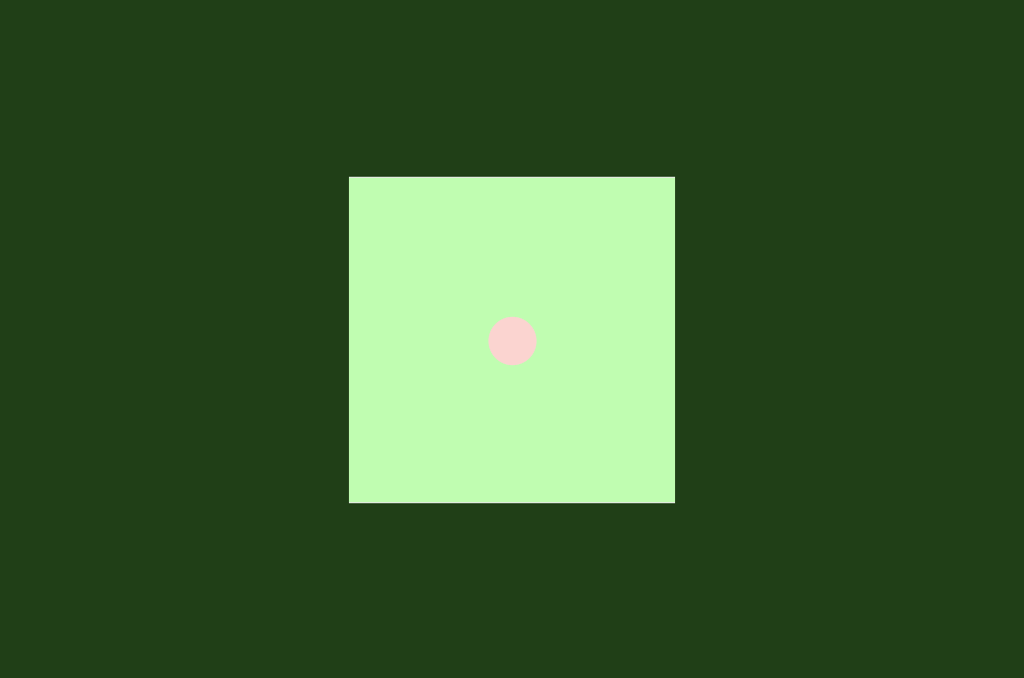
\includegraphics[width=0.5\textwidth]{a8/induction_nb}}
\caption{Die Abbildung zeigt nachgestellt das gesehene Nachbild von \textit{Induction}}
\label{induction_nb}
\end{figure}

Das erste Bild von \textit{Desaturation by Adaption} (siehe Abb. \ref{desat}) ruft im zweiten Schritt ein Nachbild hervor, in dem die ehemals gelbe Hälfte gräulich, also ungesättigter wirkt als die ehemals graue Hälfte, die quasi leuchtet (siehe Abb. \ref{desat_nb}. 

\begin{figure}[H]
\makebox[0.5\textwidth][c]{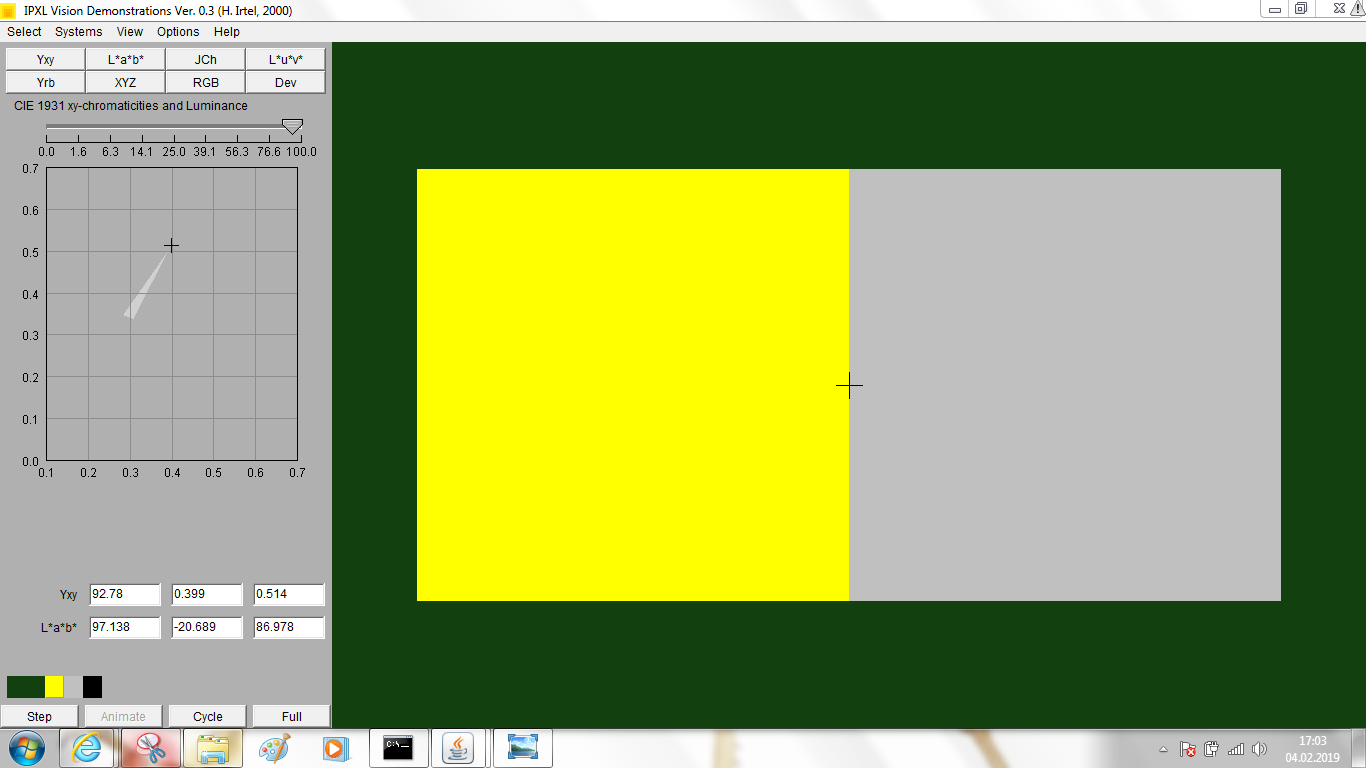
\includegraphics[width=0.5\textwidth]{a8/desaturation}}
\makebox[0.5\textwidth][c]{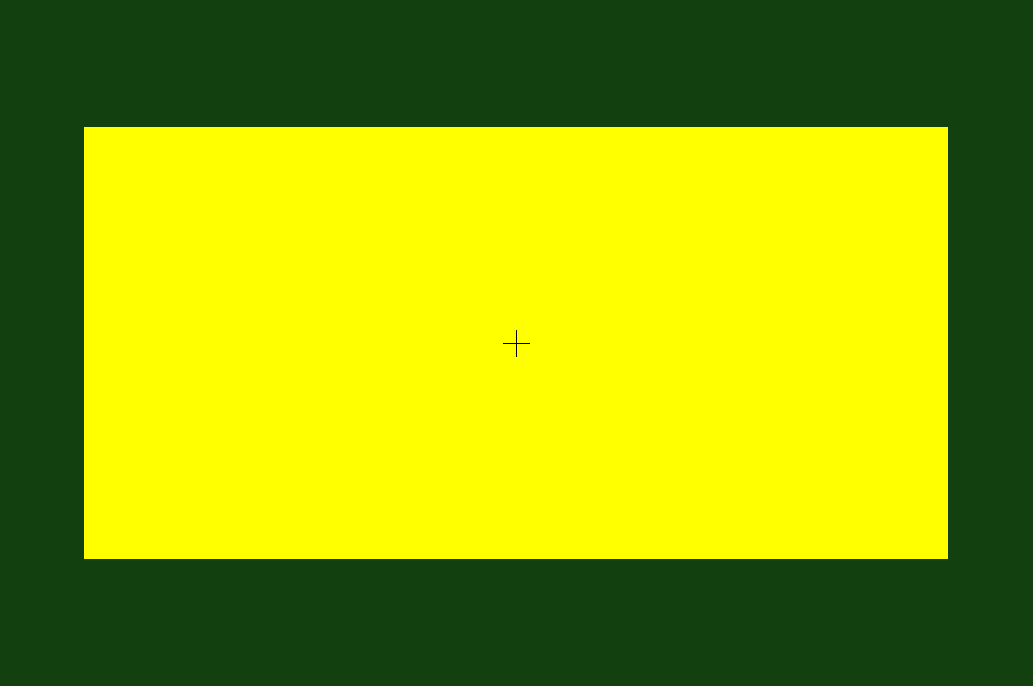
\includegraphics[width=0.5\textwidth]{a8/desaturation2}}
\caption{In der Abbildung sind die Bilder \textit{Desaturation by Adaption} sichtbar. Zuerst (links) ist das sichtbare Rechteck in der Hälfte geteilt, links ist die Fläche gelb, rechts hellgrau. Im zweiten Schritt (rechts) ist das komplette Rechteck gelb gefärbt.}
\label{desat}
\end{figure}

\begin{figure}[H]
\makebox[\textwidth][c]{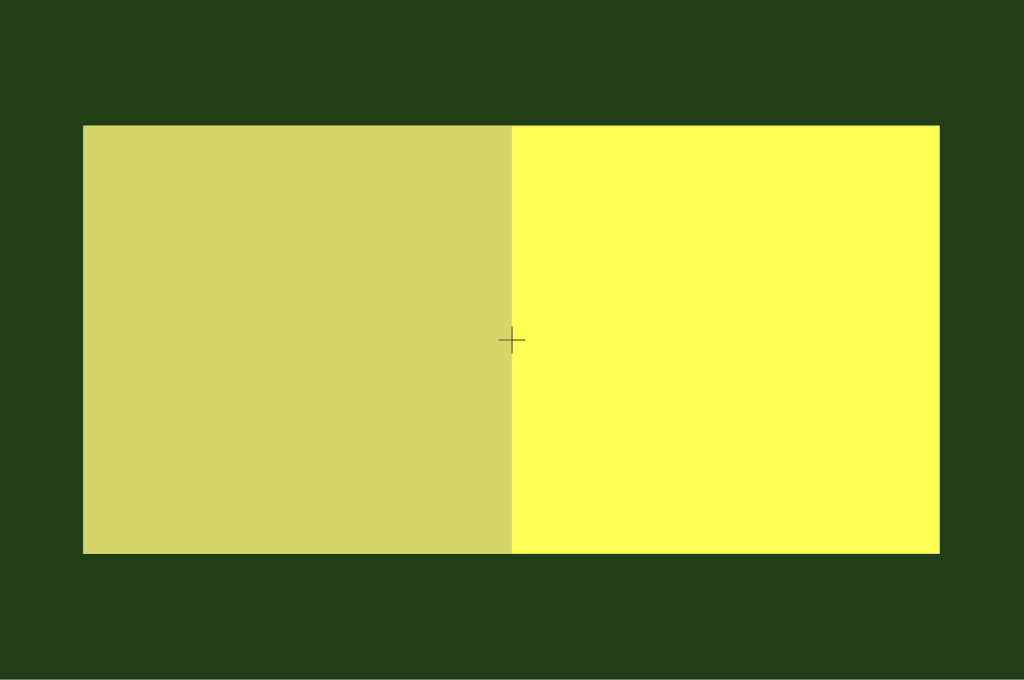
\includegraphics[width=0.5\textwidth]{a8/desat_nb}}
\caption{Die Abbildung zeigt nachgestellt das gesehene Nachbild von \textit{Desaturation by Adaption}}
\label{desat_nb}
\end{figure}

\begin{figure}[H]
\makebox[0.5\textwidth][c]{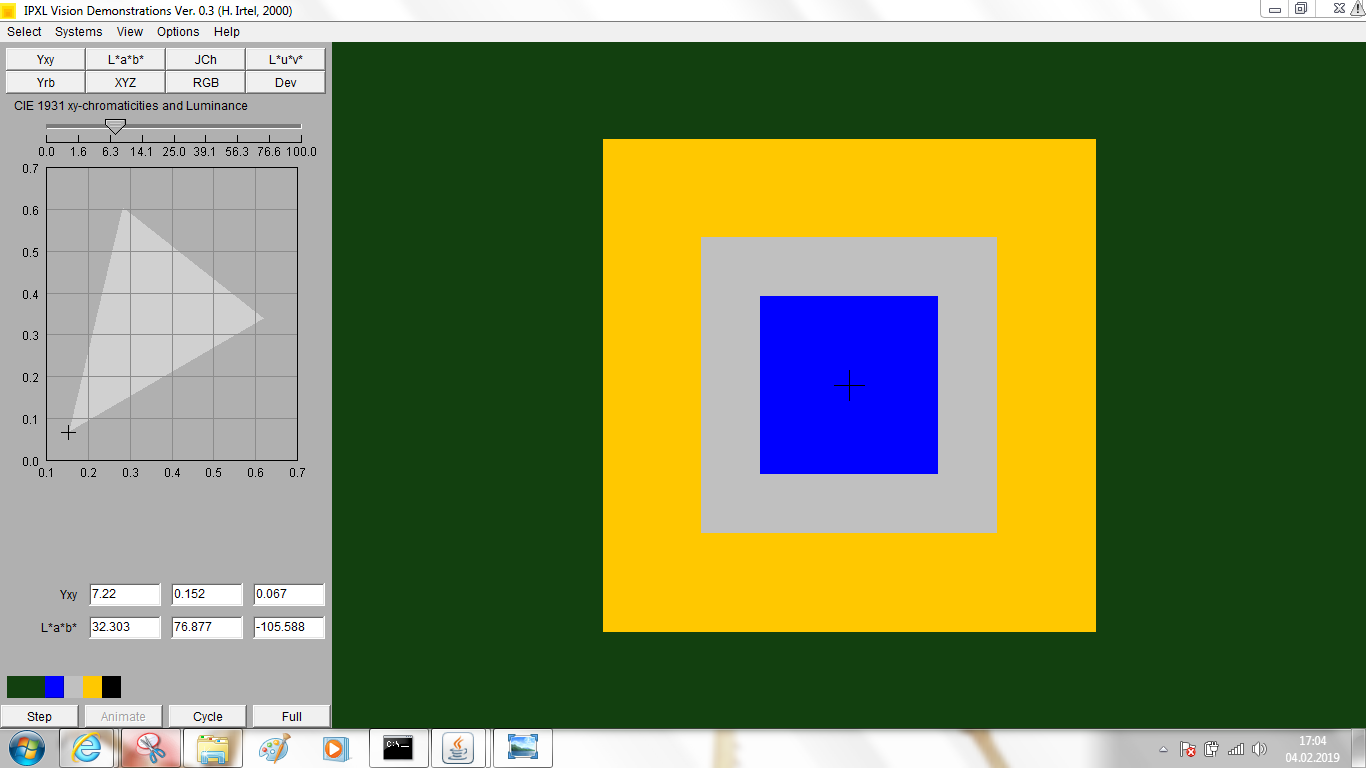
\includegraphics[width=0.5\textwidth]{a8/hypersat}}
\makebox[0.5\textwidth][c]{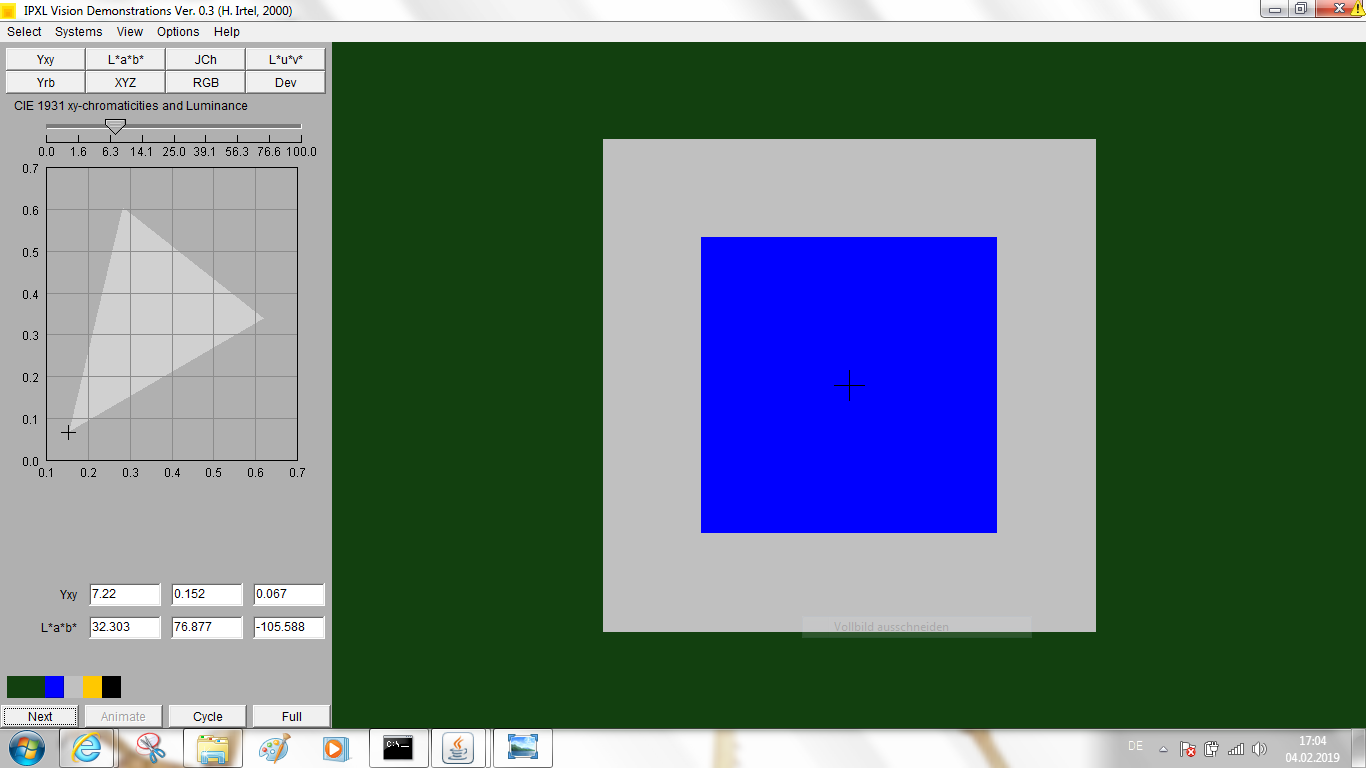
\includegraphics[width=0.5\textwidth]{a8/hypersat2}}\\ 
\makebox[0.25\textwidth][c]{}
\makebox[0.5\textwidth][c]{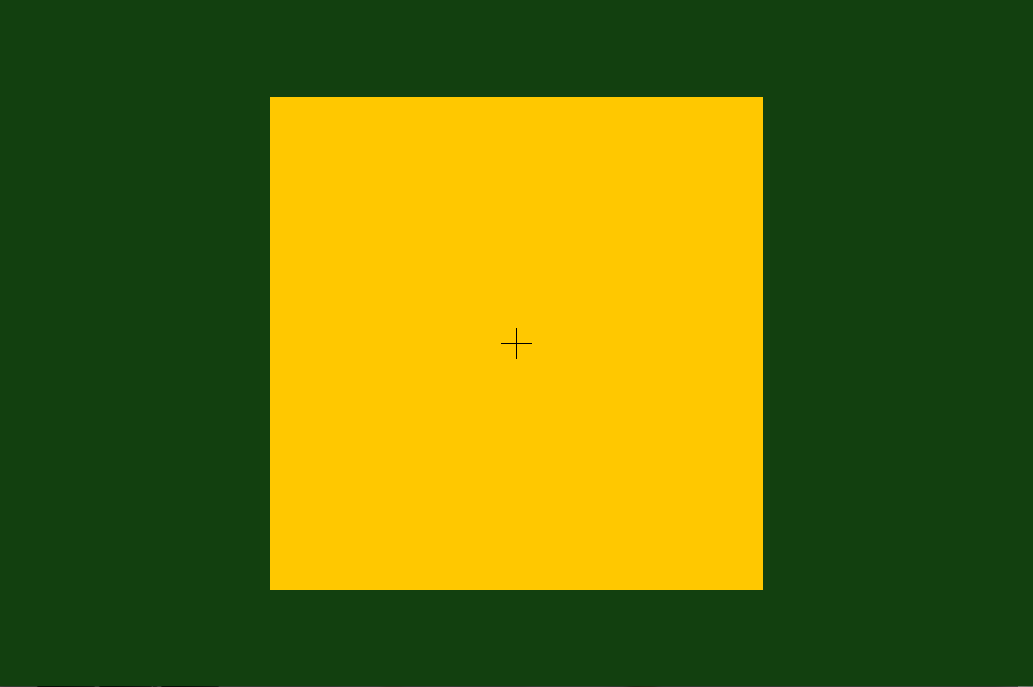
\includegraphics[width=0.5\textwidth]{a8/hypersat3}}
\caption{In der Abbildung sind die drei Bilder \textit{Hypersaturation} dargestellt. Im ersten (oben links) ist ein dreifarbiges Quadrat zu erkennen. Ganz außen ist es gelb gerahmt, die mittlere Partie ist grau und im Inneren ist ein kleineres blaues Quadrat. Im zweiten Schritt (oben rechts) hat das Quadrat nur noch zwei Farben, eine blaue Mitte und einen grauen Rand und im letzten Bild (unten) ist es komplett gelb.}
\label{hypersat}
\end{figure}

Im letzten Abschnitt dieses Versuchsteils \textit{Hypersaturation} (siehe Abb. \ref{hypersat}) wurden zwei Schritte des Nachbilds betrachtet. Nach dem Fokussieren des ersten Bildes (Abb. \ref{hypersat} l. o.) erscheint der graue Rahmen des zweiten Bildes (Abb. \ref{hypersat} r. o.) lila (s. Abb. \ref{hypersat_nb} links) und im dritten Bild (Abb. \ref{hypersat} u.) ist wieder die Dreiteilung des ersten Bildes zu erkennen, allerdings in verschieden gesättigtem Gelb. Die höchste Sättigung hat das Quadrat in der Mitte, nach außen hin nimmt die Sättigung ab. (s. Abb. \ref{hypersat_nb} rechts)  \\

\begin{figure}[H]
\makebox[0.5\textwidth][c]{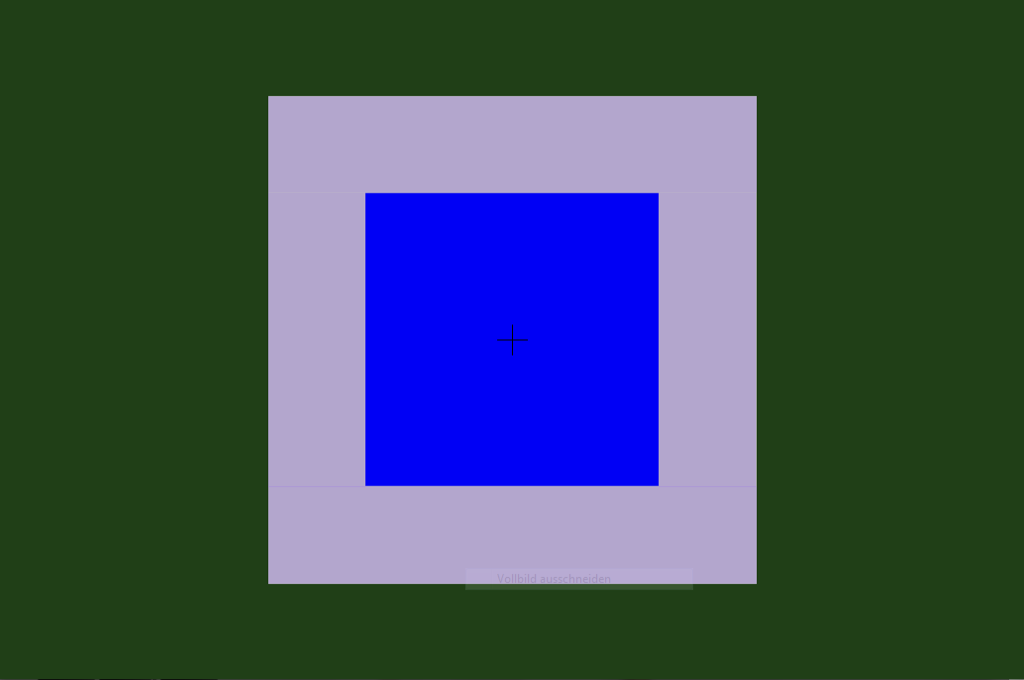
\includegraphics[width=0.5\textwidth]{a8/hypersat_nb1}}
\makebox[0.5\textwidth][c]{
\includegraphics[width=0.5\textwidth]{a8/hypersat_nb2}}
\caption{Zu sehen sind die nachgestellten Nachbilder von \textit{Hypersaturation}.}
\label{hypersat_nb}
\end{figure}

Die Entstehung von Nachbildern ist auf die lange und gleichmäßige Reizung der lichtempfindlichen Rezeptorzellen im Auge zurückzuführen. Bei dieser wird das Farbpigment aufgebraucht, so dass es an an genau an den Stellen fehlt, an dem die Rezeptorzellen farbigen Reizen ausgeliefert waren. Es entsteht der Eindruck der Komplementärfarbe.


\end{document}